% **************************************************************************************************************
% A Classic Thesis Style
% An Homage to The Elements of Typographic Style
%
% Copyright (C) 2015 André Miede http://www.miede.de
%
% If you like the style then I would appreciate a postcard. My address
% can be found in the file ClassicThesis.pdf. A collection of the
% postcards I received so far is available online at
% http://postcards.miede.de
%
% License:
% This program is free software; you can redistribute it and/or modify
% it under the terms of the GNU General Public License as published by
% the Free Software Foundation; either version 2 of the License, or
% (at your option) any later version.
%
% This program is distributed in the hope that it will be useful,
% but WITHOUT ANY WARRANTY; without even the implied warranty of
% MERCHANTABILITY or FITNESS FOR A PARTICULAR PURPOSE.  See the
% GNU General Public License for more details.
%
% You should have received a copy of the GNU General Public License
% along with this program; see the file COPYING.  If not, write to
% the Free Software Foundation, Inc., 59 Temple Place - Suite 330,
% Boston, MA 02111-1307, USA.
%
% **************************************************************************************************************
\RequirePackage{fix-cm} % fix some latex issues see: http://texdoc.net/texmf-dist/doc/latex/base/fixltx2e.pdf
\documentclass[ twoside,openright,titlepage,numbers=noenddot,headinclude,%1headlines,% letterpaper a4paper
                footinclude=true,cleardoublepage=empty,abstractoff, % <--- obsolete, remove (todo)
                BCOR=5mm,paper=a4,fontsize=11pt,%11pt,a4paper,%
                american,spanish%
                ]{scrreprt}

%********************************************************************
% Note: Make all your adjustments in here
%*******************************************************
% ****************************************************************************************************
% classicthesis-config.tex
% formerly known as loadpackages.sty, classicthesis-ldpkg.sty, and classicthesis-preamble.sty
% Use it at the beginning of your ClassicThesis.tex, or as a LaTeX Preamble
% in your ClassicThesis.{tex,lyx} with % ****************************************************************************************************
% classicthesis-config.tex
% formerly known as loadpackages.sty, classicthesis-ldpkg.sty, and classicthesis-preamble.sty
% Use it at the beginning of your ClassicThesis.tex, or as a LaTeX Preamble
% in your ClassicThesis.{tex,lyx} with % ****************************************************************************************************
% classicthesis-config.tex
% formerly known as loadpackages.sty, classicthesis-ldpkg.sty, and classicthesis-preamble.sty
% Use it at the beginning of your ClassicThesis.tex, or as a LaTeX Preamble
% in your ClassicThesis.{tex,lyx} with \input{classicthesis-config}
% ****************************************************************************************************
% If you like the classicthesis, then I would appreciate a postcard.
% My address can be found in the file ClassicThesis.pdf. A collection
% of the postcards I received so far is available online at
% http://postcards.miede.de
% ****************************************************************************************************


% ****************************************************************************************************
% 0. Set the encoding of your files. UTF-8 is the only sensible encoding nowadays. If you can't read
% äöüßáéçèê∂åëæƒÏ€ then change the encoding setting in your editor, not the line below. If your editor
% does not support utf8 use another editor!
% ****************************************************************************************************
\PassOptionsToPackage{utf8}{inputenc}
	\usepackage{inputenc}

% ****************************************************************************************************
% 1. Configure classicthesis for your needs here, e.g., remove "drafting" below
% in order to deactivate the time-stamp on the pages
% ****************************************************************************************************
\PassOptionsToPackage{eulerchapternumbers,listings,%drafting,%
					 pdfspacing,%floatperchapter,%linedheaders,%
					 subfig,beramono,eulermath,parts}{classicthesis}
% ********************************************************************
% Available options for classicthesis.sty
% (see ClassicThesis.pdf for more information):
% drafting
% parts nochapters linedheaders
% eulerchapternumbers beramono eulermath pdfspacing minionprospacing
% tocaligned dottedtoc manychapters
% listings floatperchapter subfig
% ********************************************************************


% ****************************************************************************************************
% 2. Personal data and user ad-hoc commands
% ****************************************************************************************************
\newcommand{\myTitle}{Curvas elípticas en criptografía\xspace}
\newcommand{\mySubtitle}{Trabajo Fin de Grado\xspace}
\newcommand{\myDegree}{Doble Grado en Ingeniería Informática y Matemáticas\xspace}
\newcommand{\myName}{Adrián Homero Ranea Robles\xspace}
\newcommand{\myNameShort}{Adrián H. Ranea Robles\xspace}
\newcommand{\myProf}{Pascual Jara\xspace}
\newcommand{\myFaculty}{Facultad de Ciencias\xspace}
\newcommand{\myOtherFaculty}{Escuela Técnica Superior De Ingenierías Informática y de Telecomunicación\xspace}
\newcommand{\myDepartment}{Departamento de Álgebra\xspace}
\newcommand{\myUni}{Universidad de Granada\xspace}
\newcommand{\myLocation}{Granada\xspace}
\newcommand{\myTime}{Julio de 2016\xspace}
%\newcommand{\myVersion}{version 1\xspace}

% ********************************************************************
% Setup, finetuning, and useful commands
% ********************************************************************
\newcounter{dummy} % necessary for correct hyperlinks (to index, bib, etc.)
\newlength{\abcd} % for ab..z string length calculation
\providecommand{\mLyX}{L\kern-.1667em\lower.25em\hbox{Y}\kern-.125emX\@}
\newcommand{\ie}{i.\,e.}
\newcommand{\Ie}{I.\,e.}
\newcommand{\eg}{e.\,g.}
\newcommand{\Eg}{E.\,g.}
% ****************************************************************************************************


% ****************************************************************************************************
% 3. Loading some handy packages
% ****************************************************************************************************
% ********************************************************************
% Packages with options that might require adjustments
% ********************************************************************
%\PassOptionsToPackage{ngerman,american}{babel}   % change this to your language(s)
% Spanish languages need extra options in order to work with this template
\PassOptionsToPackage{es-tabla,spanish,es-lcroman}{babel}
	\usepackage{babel}

\usepackage{csquotes}
\PassOptionsToPackage{%
    backend=biber, %instead of bibtex
	%backend=bibtex8,bibencoding=ascii,%
	language=auto,%
	%style=numeric-comp,%
    %style=authoryear-comp, % Author 1999, 2010
    %bibstyle=authoryear,dashed=false, % dashed: substitute rep. author with ---
    sorting=nyt, % name, year, title
    maxbibnames=10, % default: 3, et al.
    %backref=true,%
    natbib=true % natbib compatibility mode (\citep and \citet still work)
}{biblatex}
    \usepackage{biblatex}

\PassOptionsToPackage{fleqn}{amsmath}       % math environments and more by the AMS
    \usepackage{amsmath}

% ********************************************************************
% General useful packages
% ********************************************************************
\PassOptionsToPackage{T1}{fontenc} % T2A for cyrillics
    \usepackage{fontenc}
\usepackage{textcomp} % fix warning with missing font shapes
\usepackage{scrhack} % fix warnings when using KOMA with listings package
\usepackage{xspace} % to get the spacing after macros right
\usepackage{mparhack} % get marginpar right
\usepackage{fixltx2e} % fixes some LaTeX stuff --> since 2015 in the LaTeX kernel (see below)
%\usepackage[latest]{latexrelease} % will be used once available in more distributions (ISSUE #107)
\PassOptionsToPackage{printonlyused,smaller}{acronym}
    \usepackage{acronym} % nice macros for handling all acronyms in the thesis
    %\renewcommand{\bflabel}[1]{{#1}\hfill} % fix the list of acronyms --> no longer working
    %\renewcommand*{\acsfont}[1]{\textsc{#1}}
    \renewcommand*{\aclabelfont}[1]{\acsfont{#1}}
% ****************************************************************************************************


% ****************************************************************************************************
% 4. Setup floats: tables, (sub)figures, and captions
% ****************************************************************************************************
\usepackage{tabularx} % better tables
    \setlength{\extrarowheight}{3pt} % increase table row height
\newcommand{\tableheadline}[1]{\multicolumn{1}{c}{\spacedlowsmallcaps{#1}}}
\newcommand{\myfloatalign}{\centering} % to be used with each float for alignment
\usepackage{caption}
% Thanks to cgnieder and Claus Lahiri
% http://tex.stackexchange.com/questions/69349/spacedlowsmallcaps-in-caption-label
% [REMOVED DUE TO OTHER PROBLEMS, SEE ISSUE #82]
%\DeclareCaptionLabelFormat{smallcaps}{\bothIfFirst{#1}{~}\MakeTextLowercase{\textsc{#2}}}
%\captionsetup{font=small,labelformat=smallcaps} % format=hang,
\captionsetup{font=small} % format=hang,
\usepackage{subfig}
% ****************************************************************************************************


% ****************************************************************************************************
% 5. Setup code listings
% ****************************************************************************************************
% \usepackage{listings}
% \lccode`~=0
% %\lstset{emph={trueIndex,root},emphstyle=\color{BlueViolet}}%\underbar} % for special keywords
% \lstset{language=[LaTeX]Tex,%C++,
%     morekeywords={PassOptionsToPackage,selectlanguage},
%     keywordstyle=\color{RoyalBlue},%\bfseries,
%     basicstyle=\small\ttfamily,
%     %identifierstyle=\color{NavyBlue},
%     commentstyle=\color{Green}\ttfamily,
%     stringstyle=\rmfamily,
%     numbers=none,%left,%
%     numberstyle=\scriptsize,%\tiny
%     stepnumber=5,
%     numbersep=8pt,
%     showstringspaces=false,
%     breaklines=true,
%     %frameround=ftff,
%     %frame=single,
%     belowcaptionskip=.75\baselineskip
%     %frame=L
% }
% ****************************************************************************************************


% ****************************************************************************************************
% 6. PDFLaTeX, hyperreferences and citation backreferences
% ****************************************************************************************************
% ********************************************************************
% Using PDFLaTeX
% ********************************************************************
\PassOptionsToPackage{pdftex,hyperfootnotes=false,pdfpagelabels}{hyperref}
    \usepackage{hyperref}  % backref linktocpage pagebackref
\pdfcompresslevel=9
\pdfadjustspacing=1
\PassOptionsToPackage{pdftex}{graphicx}
    \usepackage{graphicx}


% ********************************************************************
% Hyperreferences
% ********************************************************************
\hypersetup{%
    %draft, % = no hyperlinking at all (useful in b/w printouts)
    colorlinks=true, linktocpage=true, pdfstartpage=3, pdfstartview=FitV,%
    % uncomment the following line if you want to have black links (e.g., for printing)
    %colorlinks=false, linktocpage=false, pdfstartpage=3, pdfstartview=FitV, pdfborder={0 0 0},%
    breaklinks=true, pdfpagemode=UseNone, pageanchor=true, pdfpagemode=UseOutlines,%
    plainpages=false, bookmarksnumbered, bookmarksopen=true, bookmarksopenlevel=1,%
    hypertexnames=true, pdfhighlight=/O,%nesting=true,%frenchlinks,%
    urlcolor=webbrown, linkcolor=RoyalBlue, citecolor=webgreen, %pagecolor=RoyalBlue,%
    %urlcolor=Black, linkcolor=Black, citecolor=Black, %pagecolor=Black,%
    pdftitle={\myTitle},%
    pdfauthor={\textcopyright\ \myName, \myUni},%
    pdfsubject={},%
    pdfkeywords={},%
    pdfcreator={pdfLaTeX},%
    pdfproducer={LaTeX with hyperref and classicthesis}%
}

% ********************************************************************
% Setup autoreferences
% ********************************************************************
% There are some issues regarding autorefnames
% http://www.ureader.de/msg/136221647.aspx
% http://www.tex.ac.uk/cgi-bin/texfaq2html?label=latexwords
% you have to redefine the makros for the
% language you use, e.g., american, ngerman
% (as chosen when loading babel/AtBeginDocument)
% ********************************************************************
\makeatletter
\@ifpackageloaded{babel}%
    {%
       \addto\extrasamerican{%
			\renewcommand*{\figureautorefname}{Figure}%
			\renewcommand*{\tableautorefname}{Table}%
			\renewcommand*{\partautorefname}{Part}%
			\renewcommand*{\chapterautorefname}{Chapter}%
			\renewcommand*{\sectionautorefname}{Section}%
			\renewcommand*{\subsectionautorefname}{Section}%
			\renewcommand*{\subsubsectionautorefname}{Section}%
                }%
       \addto\extrasnspanish{%
			\renewcommand*{\paragraphautorefname}{Párafro}%
			\renewcommand*{\subparagraphautorefname}{Subpárafro}%
			\renewcommand*{\footnoteautorefname}{Pie de página}%
			\renewcommand*{\FancyVerbLineautorefname}{LíneaFancy}%
			\renewcommand*{\theoremautorefname}{Teorema}%
			\renewcommand*{\appendixautorefname}{Apéndice}%
			\renewcommand*{\equationautorefname}{Ecuación}%
			\renewcommand*{\itemautorefname}{Item}%
                }%
            % Fix to getting autorefs for subfigures right (thanks to Belinda Vogt for changing the definition)
            \providecommand{\subfigureautorefname}{\figureautorefname}%
    }{\relax}
\makeatother


% ****************************************************************************************************
% 7. Last calls before the bar closes
% ****************************************************************************************************
% ********************************************************************
% Development Stuff
% ********************************************************************
%\listfiles
%\PassOptionsToPackage{l2tabu,orthodox,abort}{nag}
%   \usepackage{nag}
%\PassOptionsToPackage{warning, all}{onlyamsmath}
%   \usepackage{onlyamsmath}

% ********************************************************************
% Last, but not least...
% ********************************************************************
\usepackage{classicthesis}
% ****************************************************************************************************


% ****************************************************************************************************
% 8. Further adjustments (experimental)
% ****************************************************************************************************
% ********************************************************************
% Changing the text area
% ********************************************************************
%\linespread{1.05} % a bit more for Palatino
%\areaset[current]{312pt}{761pt} % 686 (factor 2.2) + 33 head + 42 head \the\footskip
%\setlength{\marginparwidth}{7em}%
%\setlength{\marginparsep}{2em}%

% ********************************************************************
% Using different fonts
% ********************************************************************
%\usepackage[oldstylenums]{kpfonts} % oldstyle notextcomp
%\usepackage[osf]{libertine}
%\usepackage[light,condensed,math]{iwona}
%\renewcommand{\sfdefault}{iwona}
%\usepackage{lmodern} % <-- no osf support :-(
%\usepackage{cfr-lm} %
%\usepackage[urw-garamond]{mathdesign} <-- no osf support :-(
%\usepackage[default,osfigures]{opensans} % scale=0.95
%\usepackage[sfdefault]{FiraSans}
% ****************************************************************************************************

% ****************************************************************************************************
% If you like the classicthesis, then I would appreciate a postcard.
% My address can be found in the file ClassicThesis.pdf. A collection
% of the postcards I received so far is available online at
% http://postcards.miede.de
% ****************************************************************************************************


% ****************************************************************************************************
% 0. Set the encoding of your files. UTF-8 is the only sensible encoding nowadays. If you can't read
% äöüßáéçèê∂åëæƒÏ€ then change the encoding setting in your editor, not the line below. If your editor
% does not support utf8 use another editor!
% ****************************************************************************************************
\PassOptionsToPackage{utf8}{inputenc}
	\usepackage{inputenc}

% ****************************************************************************************************
% 1. Configure classicthesis for your needs here, e.g., remove "drafting" below
% in order to deactivate the time-stamp on the pages
% ****************************************************************************************************
\PassOptionsToPackage{eulerchapternumbers,listings,%drafting,%
					 pdfspacing,%floatperchapter,%linedheaders,%
					 subfig,beramono,eulermath,parts}{classicthesis}
% ********************************************************************
% Available options for classicthesis.sty
% (see ClassicThesis.pdf for more information):
% drafting
% parts nochapters linedheaders
% eulerchapternumbers beramono eulermath pdfspacing minionprospacing
% tocaligned dottedtoc manychapters
% listings floatperchapter subfig
% ********************************************************************


% ****************************************************************************************************
% 2. Personal data and user ad-hoc commands
% ****************************************************************************************************
\newcommand{\myTitle}{Curvas elípticas en criptografía\xspace}
\newcommand{\mySubtitle}{Trabajo Fin de Grado\xspace}
\newcommand{\myDegree}{Doble Grado en Ingeniería Informática y Matemáticas\xspace}
\newcommand{\myName}{Adrián Homero Ranea Robles\xspace}
\newcommand{\myNameShort}{Adrián H. Ranea Robles\xspace}
\newcommand{\myProf}{Pascual Jara\xspace}
\newcommand{\myFaculty}{Facultad de Ciencias\xspace}
\newcommand{\myOtherFaculty}{Escuela Técnica Superior De Ingenierías Informática y de Telecomunicación\xspace}
\newcommand{\myDepartment}{Departamento de Álgebra\xspace}
\newcommand{\myUni}{Universidad de Granada\xspace}
\newcommand{\myLocation}{Granada\xspace}
\newcommand{\myTime}{Julio de 2016\xspace}
%\newcommand{\myVersion}{version 1\xspace}

% ********************************************************************
% Setup, finetuning, and useful commands
% ********************************************************************
\newcounter{dummy} % necessary for correct hyperlinks (to index, bib, etc.)
\newlength{\abcd} % for ab..z string length calculation
\providecommand{\mLyX}{L\kern-.1667em\lower.25em\hbox{Y}\kern-.125emX\@}
\newcommand{\ie}{i.\,e.}
\newcommand{\Ie}{I.\,e.}
\newcommand{\eg}{e.\,g.}
\newcommand{\Eg}{E.\,g.}
% ****************************************************************************************************


% ****************************************************************************************************
% 3. Loading some handy packages
% ****************************************************************************************************
% ********************************************************************
% Packages with options that might require adjustments
% ********************************************************************
%\PassOptionsToPackage{ngerman,american}{babel}   % change this to your language(s)
% Spanish languages need extra options in order to work with this template
\PassOptionsToPackage{es-tabla,spanish,es-lcroman}{babel}
	\usepackage{babel}

\usepackage{csquotes}
\PassOptionsToPackage{%
    backend=biber, %instead of bibtex
	%backend=bibtex8,bibencoding=ascii,%
	language=auto,%
	%style=numeric-comp,%
    %style=authoryear-comp, % Author 1999, 2010
    %bibstyle=authoryear,dashed=false, % dashed: substitute rep. author with ---
    sorting=nyt, % name, year, title
    maxbibnames=10, % default: 3, et al.
    %backref=true,%
    natbib=true % natbib compatibility mode (\citep and \citet still work)
}{biblatex}
    \usepackage{biblatex}

\PassOptionsToPackage{fleqn}{amsmath}       % math environments and more by the AMS
    \usepackage{amsmath}

% ********************************************************************
% General useful packages
% ********************************************************************
\PassOptionsToPackage{T1}{fontenc} % T2A for cyrillics
    \usepackage{fontenc}
\usepackage{textcomp} % fix warning with missing font shapes
\usepackage{scrhack} % fix warnings when using KOMA with listings package
\usepackage{xspace} % to get the spacing after macros right
\usepackage{mparhack} % get marginpar right
\usepackage{fixltx2e} % fixes some LaTeX stuff --> since 2015 in the LaTeX kernel (see below)
%\usepackage[latest]{latexrelease} % will be used once available in more distributions (ISSUE #107)
\PassOptionsToPackage{printonlyused,smaller}{acronym}
    \usepackage{acronym} % nice macros for handling all acronyms in the thesis
    %\renewcommand{\bflabel}[1]{{#1}\hfill} % fix the list of acronyms --> no longer working
    %\renewcommand*{\acsfont}[1]{\textsc{#1}}
    \renewcommand*{\aclabelfont}[1]{\acsfont{#1}}
% ****************************************************************************************************


% ****************************************************************************************************
% 4. Setup floats: tables, (sub)figures, and captions
% ****************************************************************************************************
\usepackage{tabularx} % better tables
    \setlength{\extrarowheight}{3pt} % increase table row height
\newcommand{\tableheadline}[1]{\multicolumn{1}{c}{\spacedlowsmallcaps{#1}}}
\newcommand{\myfloatalign}{\centering} % to be used with each float for alignment
\usepackage{caption}
% Thanks to cgnieder and Claus Lahiri
% http://tex.stackexchange.com/questions/69349/spacedlowsmallcaps-in-caption-label
% [REMOVED DUE TO OTHER PROBLEMS, SEE ISSUE #82]
%\DeclareCaptionLabelFormat{smallcaps}{\bothIfFirst{#1}{~}\MakeTextLowercase{\textsc{#2}}}
%\captionsetup{font=small,labelformat=smallcaps} % format=hang,
\captionsetup{font=small} % format=hang,
\usepackage{subfig}
% ****************************************************************************************************


% ****************************************************************************************************
% 5. Setup code listings
% ****************************************************************************************************
% \usepackage{listings}
% \lccode`~=0
% %\lstset{emph={trueIndex,root},emphstyle=\color{BlueViolet}}%\underbar} % for special keywords
% \lstset{language=[LaTeX]Tex,%C++,
%     morekeywords={PassOptionsToPackage,selectlanguage},
%     keywordstyle=\color{RoyalBlue},%\bfseries,
%     basicstyle=\small\ttfamily,
%     %identifierstyle=\color{NavyBlue},
%     commentstyle=\color{Green}\ttfamily,
%     stringstyle=\rmfamily,
%     numbers=none,%left,%
%     numberstyle=\scriptsize,%\tiny
%     stepnumber=5,
%     numbersep=8pt,
%     showstringspaces=false,
%     breaklines=true,
%     %frameround=ftff,
%     %frame=single,
%     belowcaptionskip=.75\baselineskip
%     %frame=L
% }
% ****************************************************************************************************


% ****************************************************************************************************
% 6. PDFLaTeX, hyperreferences and citation backreferences
% ****************************************************************************************************
% ********************************************************************
% Using PDFLaTeX
% ********************************************************************
\PassOptionsToPackage{pdftex,hyperfootnotes=false,pdfpagelabels}{hyperref}
    \usepackage{hyperref}  % backref linktocpage pagebackref
\pdfcompresslevel=9
\pdfadjustspacing=1
\PassOptionsToPackage{pdftex}{graphicx}
    \usepackage{graphicx}


% ********************************************************************
% Hyperreferences
% ********************************************************************
\hypersetup{%
    %draft, % = no hyperlinking at all (useful in b/w printouts)
    colorlinks=true, linktocpage=true, pdfstartpage=3, pdfstartview=FitV,%
    % uncomment the following line if you want to have black links (e.g., for printing)
    %colorlinks=false, linktocpage=false, pdfstartpage=3, pdfstartview=FitV, pdfborder={0 0 0},%
    breaklinks=true, pdfpagemode=UseNone, pageanchor=true, pdfpagemode=UseOutlines,%
    plainpages=false, bookmarksnumbered, bookmarksopen=true, bookmarksopenlevel=1,%
    hypertexnames=true, pdfhighlight=/O,%nesting=true,%frenchlinks,%
    urlcolor=webbrown, linkcolor=RoyalBlue, citecolor=webgreen, %pagecolor=RoyalBlue,%
    %urlcolor=Black, linkcolor=Black, citecolor=Black, %pagecolor=Black,%
    pdftitle={\myTitle},%
    pdfauthor={\textcopyright\ \myName, \myUni},%
    pdfsubject={},%
    pdfkeywords={},%
    pdfcreator={pdfLaTeX},%
    pdfproducer={LaTeX with hyperref and classicthesis}%
}

% ********************************************************************
% Setup autoreferences
% ********************************************************************
% There are some issues regarding autorefnames
% http://www.ureader.de/msg/136221647.aspx
% http://www.tex.ac.uk/cgi-bin/texfaq2html?label=latexwords
% you have to redefine the makros for the
% language you use, e.g., american, ngerman
% (as chosen when loading babel/AtBeginDocument)
% ********************************************************************
\makeatletter
\@ifpackageloaded{babel}%
    {%
       \addto\extrasamerican{%
			\renewcommand*{\figureautorefname}{Figure}%
			\renewcommand*{\tableautorefname}{Table}%
			\renewcommand*{\partautorefname}{Part}%
			\renewcommand*{\chapterautorefname}{Chapter}%
			\renewcommand*{\sectionautorefname}{Section}%
			\renewcommand*{\subsectionautorefname}{Section}%
			\renewcommand*{\subsubsectionautorefname}{Section}%
                }%
       \addto\extrasnspanish{%
			\renewcommand*{\paragraphautorefname}{Párafro}%
			\renewcommand*{\subparagraphautorefname}{Subpárafro}%
			\renewcommand*{\footnoteautorefname}{Pie de página}%
			\renewcommand*{\FancyVerbLineautorefname}{LíneaFancy}%
			\renewcommand*{\theoremautorefname}{Teorema}%
			\renewcommand*{\appendixautorefname}{Apéndice}%
			\renewcommand*{\equationautorefname}{Ecuación}%
			\renewcommand*{\itemautorefname}{Item}%
                }%
            % Fix to getting autorefs for subfigures right (thanks to Belinda Vogt for changing the definition)
            \providecommand{\subfigureautorefname}{\figureautorefname}%
    }{\relax}
\makeatother


% ****************************************************************************************************
% 7. Last calls before the bar closes
% ****************************************************************************************************
% ********************************************************************
% Development Stuff
% ********************************************************************
%\listfiles
%\PassOptionsToPackage{l2tabu,orthodox,abort}{nag}
%   \usepackage{nag}
%\PassOptionsToPackage{warning, all}{onlyamsmath}
%   \usepackage{onlyamsmath}

% ********************************************************************
% Last, but not least...
% ********************************************************************
\usepackage{classicthesis}
% ****************************************************************************************************


% ****************************************************************************************************
% 8. Further adjustments (experimental)
% ****************************************************************************************************
% ********************************************************************
% Changing the text area
% ********************************************************************
%\linespread{1.05} % a bit more for Palatino
%\areaset[current]{312pt}{761pt} % 686 (factor 2.2) + 33 head + 42 head \the\footskip
%\setlength{\marginparwidth}{7em}%
%\setlength{\marginparsep}{2em}%

% ********************************************************************
% Using different fonts
% ********************************************************************
%\usepackage[oldstylenums]{kpfonts} % oldstyle notextcomp
%\usepackage[osf]{libertine}
%\usepackage[light,condensed,math]{iwona}
%\renewcommand{\sfdefault}{iwona}
%\usepackage{lmodern} % <-- no osf support :-(
%\usepackage{cfr-lm} %
%\usepackage[urw-garamond]{mathdesign} <-- no osf support :-(
%\usepackage[default,osfigures]{opensans} % scale=0.95
%\usepackage[sfdefault]{FiraSans}
% ****************************************************************************************************

% ****************************************************************************************************
% If you like the classicthesis, then I would appreciate a postcard.
% My address can be found in the file ClassicThesis.pdf. A collection
% of the postcards I received so far is available online at
% http://postcards.miede.de
% ****************************************************************************************************


% ****************************************************************************************************
% 0. Set the encoding of your files. UTF-8 is the only sensible encoding nowadays. If you can't read
% äöüßáéçèê∂åëæƒÏ€ then change the encoding setting in your editor, not the line below. If your editor
% does not support utf8 use another editor!
% ****************************************************************************************************
\PassOptionsToPackage{utf8}{inputenc}
	\usepackage{inputenc}

% ****************************************************************************************************
% 1. Configure classicthesis for your needs here, e.g., remove "drafting" below
% in order to deactivate the time-stamp on the pages
% ****************************************************************************************************
\PassOptionsToPackage{eulerchapternumbers,listings,%drafting,%
					 pdfspacing,%floatperchapter,%linedheaders,%
					 subfig,beramono,eulermath,parts}{classicthesis}
% ********************************************************************
% Available options for classicthesis.sty
% (see ClassicThesis.pdf for more information):
% drafting
% parts nochapters linedheaders
% eulerchapternumbers beramono eulermath pdfspacing minionprospacing
% tocaligned dottedtoc manychapters
% listings floatperchapter subfig
% ********************************************************************


% ****************************************************************************************************
% 2. Personal data and user ad-hoc commands
% ****************************************************************************************************
\newcommand{\myTitle}{Curvas elípticas en criptografía\xspace}
\newcommand{\mySubtitle}{Trabajo Fin de Grado\xspace}
\newcommand{\myDegree}{Doble Grado en Ingeniería Informática y Matemáticas\xspace}
\newcommand{\myName}{Adrián Homero Ranea Robles\xspace}
\newcommand{\myNameShort}{Adrián H. Ranea Robles\xspace}
\newcommand{\myProf}{Pascual Jara\xspace}
\newcommand{\myFaculty}{Facultad de Ciencias\xspace}
\newcommand{\myOtherFaculty}{Escuela Técnica Superior De Ingenierías Informática y de Telecomunicación\xspace}
\newcommand{\myDepartment}{Departamento de Álgebra\xspace}
\newcommand{\myUni}{Universidad de Granada\xspace}
\newcommand{\myLocation}{Granada\xspace}
\newcommand{\myTime}{Julio de 2016\xspace}
%\newcommand{\myVersion}{version 1\xspace}

% ********************************************************************
% Setup, finetuning, and useful commands
% ********************************************************************
\newcounter{dummy} % necessary for correct hyperlinks (to index, bib, etc.)
\newlength{\abcd} % for ab..z string length calculation
\providecommand{\mLyX}{L\kern-.1667em\lower.25em\hbox{Y}\kern-.125emX\@}
\newcommand{\ie}{i.\,e.}
\newcommand{\Ie}{I.\,e.}
\newcommand{\eg}{e.\,g.}
\newcommand{\Eg}{E.\,g.}
% ****************************************************************************************************


% ****************************************************************************************************
% 3. Loading some handy packages
% ****************************************************************************************************
% ********************************************************************
% Packages with options that might require adjustments
% ********************************************************************
%\PassOptionsToPackage{ngerman,american}{babel}   % change this to your language(s)
% Spanish languages need extra options in order to work with this template
\PassOptionsToPackage{es-tabla,spanish,es-lcroman}{babel}
	\usepackage{babel}

\usepackage{csquotes}
\PassOptionsToPackage{%
    backend=biber, %instead of bibtex
	%backend=bibtex8,bibencoding=ascii,%
	language=auto,%
	%style=numeric-comp,%
    %style=authoryear-comp, % Author 1999, 2010
    %bibstyle=authoryear,dashed=false, % dashed: substitute rep. author with ---
    sorting=nyt, % name, year, title
    maxbibnames=10, % default: 3, et al.
    %backref=true,%
    natbib=true % natbib compatibility mode (\citep and \citet still work)
}{biblatex}
    \usepackage{biblatex}

\PassOptionsToPackage{fleqn}{amsmath}       % math environments and more by the AMS
    \usepackage{amsmath}

% ********************************************************************
% General useful packages
% ********************************************************************
\PassOptionsToPackage{T1}{fontenc} % T2A for cyrillics
    \usepackage{fontenc}
\usepackage{textcomp} % fix warning with missing font shapes
\usepackage{scrhack} % fix warnings when using KOMA with listings package
\usepackage{xspace} % to get the spacing after macros right
\usepackage{mparhack} % get marginpar right
\usepackage{fixltx2e} % fixes some LaTeX stuff --> since 2015 in the LaTeX kernel (see below)
%\usepackage[latest]{latexrelease} % will be used once available in more distributions (ISSUE #107)
\PassOptionsToPackage{printonlyused,smaller}{acronym}
    \usepackage{acronym} % nice macros for handling all acronyms in the thesis
    %\renewcommand{\bflabel}[1]{{#1}\hfill} % fix the list of acronyms --> no longer working
    %\renewcommand*{\acsfont}[1]{\textsc{#1}}
    \renewcommand*{\aclabelfont}[1]{\acsfont{#1}}
% ****************************************************************************************************


% ****************************************************************************************************
% 4. Setup floats: tables, (sub)figures, and captions
% ****************************************************************************************************
\usepackage{tabularx} % better tables
    \setlength{\extrarowheight}{3pt} % increase table row height
\newcommand{\tableheadline}[1]{\multicolumn{1}{c}{\spacedlowsmallcaps{#1}}}
\newcommand{\myfloatalign}{\centering} % to be used with each float for alignment
\usepackage{caption}
% Thanks to cgnieder and Claus Lahiri
% http://tex.stackexchange.com/questions/69349/spacedlowsmallcaps-in-caption-label
% [REMOVED DUE TO OTHER PROBLEMS, SEE ISSUE #82]
%\DeclareCaptionLabelFormat{smallcaps}{\bothIfFirst{#1}{~}\MakeTextLowercase{\textsc{#2}}}
%\captionsetup{font=small,labelformat=smallcaps} % format=hang,
\captionsetup{font=small} % format=hang,
\usepackage{subfig}
% ****************************************************************************************************


% ****************************************************************************************************
% 5. Setup code listings
% ****************************************************************************************************
% \usepackage{listings}
% \lccode`~=0
% %\lstset{emph={trueIndex,root},emphstyle=\color{BlueViolet}}%\underbar} % for special keywords
% \lstset{language=[LaTeX]Tex,%C++,
%     morekeywords={PassOptionsToPackage,selectlanguage},
%     keywordstyle=\color{RoyalBlue},%\bfseries,
%     basicstyle=\small\ttfamily,
%     %identifierstyle=\color{NavyBlue},
%     commentstyle=\color{Green}\ttfamily,
%     stringstyle=\rmfamily,
%     numbers=none,%left,%
%     numberstyle=\scriptsize,%\tiny
%     stepnumber=5,
%     numbersep=8pt,
%     showstringspaces=false,
%     breaklines=true,
%     %frameround=ftff,
%     %frame=single,
%     belowcaptionskip=.75\baselineskip
%     %frame=L
% }
% ****************************************************************************************************


% ****************************************************************************************************
% 6. PDFLaTeX, hyperreferences and citation backreferences
% ****************************************************************************************************
% ********************************************************************
% Using PDFLaTeX
% ********************************************************************
\PassOptionsToPackage{pdftex,hyperfootnotes=false,pdfpagelabels}{hyperref}
    \usepackage{hyperref}  % backref linktocpage pagebackref
\pdfcompresslevel=9
\pdfadjustspacing=1
\PassOptionsToPackage{pdftex}{graphicx}
    \usepackage{graphicx}


% ********************************************************************
% Hyperreferences
% ********************************************************************
\hypersetup{%
    %draft, % = no hyperlinking at all (useful in b/w printouts)
    colorlinks=true, linktocpage=true, pdfstartpage=3, pdfstartview=FitV,%
    % uncomment the following line if you want to have black links (e.g., for printing)
    %colorlinks=false, linktocpage=false, pdfstartpage=3, pdfstartview=FitV, pdfborder={0 0 0},%
    breaklinks=true, pdfpagemode=UseNone, pageanchor=true, pdfpagemode=UseOutlines,%
    plainpages=false, bookmarksnumbered, bookmarksopen=true, bookmarksopenlevel=1,%
    hypertexnames=true, pdfhighlight=/O,%nesting=true,%frenchlinks,%
    urlcolor=webbrown, linkcolor=RoyalBlue, citecolor=webgreen, %pagecolor=RoyalBlue,%
    %urlcolor=Black, linkcolor=Black, citecolor=Black, %pagecolor=Black,%
    pdftitle={\myTitle},%
    pdfauthor={\textcopyright\ \myName, \myUni},%
    pdfsubject={},%
    pdfkeywords={},%
    pdfcreator={pdfLaTeX},%
    pdfproducer={LaTeX with hyperref and classicthesis}%
}

% ********************************************************************
% Setup autoreferences
% ********************************************************************
% There are some issues regarding autorefnames
% http://www.ureader.de/msg/136221647.aspx
% http://www.tex.ac.uk/cgi-bin/texfaq2html?label=latexwords
% you have to redefine the makros for the
% language you use, e.g., american, ngerman
% (as chosen when loading babel/AtBeginDocument)
% ********************************************************************
\makeatletter
\@ifpackageloaded{babel}%
    {%
       \addto\extrasamerican{%
			\renewcommand*{\figureautorefname}{Figure}%
			\renewcommand*{\tableautorefname}{Table}%
			\renewcommand*{\partautorefname}{Part}%
			\renewcommand*{\chapterautorefname}{Chapter}%
			\renewcommand*{\sectionautorefname}{Section}%
			\renewcommand*{\subsectionautorefname}{Section}%
			\renewcommand*{\subsubsectionautorefname}{Section}%
                }%
       \addto\extrasnspanish{%
			\renewcommand*{\paragraphautorefname}{Párafro}%
			\renewcommand*{\subparagraphautorefname}{Subpárafro}%
			\renewcommand*{\footnoteautorefname}{Pie de página}%
			\renewcommand*{\FancyVerbLineautorefname}{LíneaFancy}%
			\renewcommand*{\theoremautorefname}{Teorema}%
			\renewcommand*{\appendixautorefname}{Apéndice}%
			\renewcommand*{\equationautorefname}{Ecuación}%
			\renewcommand*{\itemautorefname}{Item}%
                }%
            % Fix to getting autorefs for subfigures right (thanks to Belinda Vogt for changing the definition)
            \providecommand{\subfigureautorefname}{\figureautorefname}%
    }{\relax}
\makeatother


% ****************************************************************************************************
% 7. Last calls before the bar closes
% ****************************************************************************************************
% ********************************************************************
% Development Stuff
% ********************************************************************
%\listfiles
%\PassOptionsToPackage{l2tabu,orthodox,abort}{nag}
%   \usepackage{nag}
%\PassOptionsToPackage{warning, all}{onlyamsmath}
%   \usepackage{onlyamsmath}

% ********************************************************************
% Last, but not least...
% ********************************************************************
\usepackage{classicthesis}
% ****************************************************************************************************


% ****************************************************************************************************
% 8. Further adjustments (experimental)
% ****************************************************************************************************
% ********************************************************************
% Changing the text area
% ********************************************************************
%\linespread{1.05} % a bit more for Palatino
%\areaset[current]{312pt}{761pt} % 686 (factor 2.2) + 33 head + 42 head \the\footskip
%\setlength{\marginparwidth}{7em}%
%\setlength{\marginparsep}{2em}%

% ********************************************************************
% Using different fonts
% ********************************************************************
%\usepackage[oldstylenums]{kpfonts} % oldstyle notextcomp
%\usepackage[osf]{libertine}
%\usepackage[light,condensed,math]{iwona}
%\renewcommand{\sfdefault}{iwona}
%\usepackage{lmodern} % <-- no osf support :-(
%\usepackage{cfr-lm} %
%\usepackage[urw-garamond]{mathdesign} <-- no osf support :-(
%\usepackage[default,osfigures]{opensans} % scale=0.95
%\usepackage[sfdefault]{FiraSans}
% ****************************************************************************************************


% # Paquetes
\usepackage{amsthm} % para usar \newtheorem y \proof
\usepackage{mathtools} % para usar rcases
\usepackage{enumitem} % pasa usar tag distintos en las enumeraciones
\usepackage{amssymb} % para usar el simbolo de no divide
\usepackage{xeboiboites} % TODO: añadir ref

% # Definición de estilos de "teoremas":
% # \newtheorem{identificador}{texto}[contador]
% \theoremstyle{plain} % titulo negrita, cuerpo cursiva
\theoremstyle{definition} % titulo negrita, cuerpo en recta
% TODO: ver que hacer
\newtheorem{contador}{contador}[chapter]
% \newtheorem{proposicion}[teorema]{Proposicion}
% \newtheorem{lema}[teorema]{Lema}
% \newtheorem{ejemplo}[teorema]{Ejemplo}
% \newtheorem{definicion}[teorema]{Definición}
% \newtheorem{nota}[teorema]{Nota}
% \newtheorem{ley de grupo}[teorema]{Ley de grupo}
% \newtheorem{algoritmo}[teorema]{Algoritmo}
% \newtheorem{corolario}[teorema]{Corolario}
\newcommand{\nuevoteorema}[3] {
    \newbreakabletheorem[small box style={draw=orange!30!black!20,%
    fill=orange!10!black!2,decoration=penciline, decorate, thick},
    big box style={color=orange!30!black!20,fill=orange!30!black!10,thick},
    broken edges={draw=orange!30!black!20,thick,fill=orange!20!black!5,
    decoration={penciline,segment length=.5cm,%
    amplitude=1.3mm},decorate},%
    other edges={decorate,thick}]%
    {#1}{#2}{#3}
}
\nuevoteorema{teorema}{Teorema}{contador}
\nuevoteorema{proposicion}{Proposición}{contador}
\nuevoteorema{lema}{Lema}{contador}
\nuevoteorema{corolario}{Corolario}{contador}
\nuevoteorema{ley de grupo}{Ley de grupo}{contador}
\nuevoteorema{definicion}{Definición}{contador}
\nuevoteorema{algoritmo}{Algoritmo}{contador}
\nuevoteorema{formulasadiccion}{Fórmulas de adicción}{contador}
%\nuevoteorema{ejemplo}{Ejemplo}{contador}
%\nuevoteorema{nota}{Nota}{contador}
\newtheorem{nota}[contador]{Nota}
\newtheorem{ejemplo}[contador]{Ejemplo}
%\newtheorem{nota}[contador]{Nota}
\nuevoteorema{protocolo}{Protocolo criptográfico}{contador}

\nuevoteorema{teorema2}{Teorema}{}
\nuevoteorema{metodocuerda}{Método de la cuerda y la tangente}{}


% # Comandos definidos
\newcommand{\F}{\mathbb{F}}
\newcommand{\Fq}{\mathbb{F}_q}
\newcommand{\Fqca}{\overline{\Fq}}
\newcommand{\Fm}{\mathbb{F}_{2^m}}
\newcommand{\Fp}{\mathbb{F}_p}
\renewcommand{\P}{\mathbb{P}}
\newcommand{\A}{\mathbb{A}}
\newcommand{\Kca}{\overline{K}}
\newcommand{\EK}{E(K)}
\newcommand{\EKca}{E(\Kca)}
\newcommand{\EFqca}{E(\Fqca)}
%\newcommand{\deg}{\textrm{deg}}
\newcommand{\dega}{\deg(\alpha)}
%\let\char\relax
\DeclareMathOperator{\car}{char}
\newcommand{\phiq}{\phi_q}


%********************************************************************
% Bibliographies
%*******************************************************
\addbibresource{Bibliography.bib}
%\addbibresource[label=ownpubs]{AMiede_Publications.bib}

%********************************************************************
% Hyphenation
%*******************************************************
%\hyphenation{put special hyphenation here}

% ********************************************************************
% GO!GO!GO! MOVE IT!
%*******************************************************
\begin{document}
\frenchspacing
\raggedbottom
\selectlanguage{spanish} % american ngerman
%\renewcommand*{\bibname}{new name}
%\setbibpreamble{}
\pagenumbering{roman}
\pagestyle{plain}
%********************************************************************
% Frontmatter
%*******************************************************
% TODO: descomentar todo menos Publications
%%*******************************************************
% Little Dirty Titlepage
%*******************************************************
\thispagestyle{empty}
%\pdfbookmark[1]{Titel}{title}
%*******************************************************
\begin{center}
    \spacedlowsmallcaps{\myName} \\ \medskip                        

    \begingroup
        \color{Maroon}\spacedallcaps{\myTitle}
    \endgroup
\end{center}        

%%*******************************************************
% Titlepage
%*******************************************************
\begin{titlepage}
    % if you want the titlepage to be centered, uncomment and fine-tune the line below (KOMA classes environment)
    \begin{addmargin}[-1cm]{-3cm}
    \begin{center}
        \large

        \hfill

        \vfill

        %
\includegraphics[width=0.9\textwidth]{gfx/logo_ugr2.png}\\[1.4cm]
        
\includegraphics[width=4cm]{gfx/logo_ugr2} %\\ \medskip

        \vfill

        \spacedallcaps{\mySubtitle} \\ \bigskip

        \spacedlowsmallcaps{\myDegree} \\ \bigskip \bigskip

        % \vfill

        \begingroup
            \color{Maroon}\spacedallcaps{\LARGE\myTitle} \\ \bigskip
        \endgroup

        \vfill

        \textbf{Autor} \\
        \myName \\ \medskip

        \textbf{Tutor} \\
        \myProf \\ \medskip

        \vfill

        %\myDepartment \\
        \spacedlowsmallcaps{\myUni} \\ \medskip
        %\spacedlowsmallcaps{\myFaculty} \\
        %\spacedlowsmallcaps{\myOtherFaculty} \\ \bigskip
        %\myUni \\ \bigskip

        \myLocation, \myTime %\ -- \myVersion

        \vfill

    \end{center}
  \end{addmargin}
\end{titlepage}

%%*******************************************************
% Titlepage
%*******************************************************
\begin{titlepage}
    % if you want the titlepage to be centered, uncomment and fine-tune the line below (KOMA classes environment)
    \begin{addmargin}[-1cm]{-3cm}
    \begin{center}
        \large

        \hfill

        \vfill

        % \vfill

        \begingroup
            \color{Maroon}\spacedallcaps{\LARGE\myTitle} \\ \bigskip
        \endgroup

        \vfill

        \textbf{Autor} \\
        \myName \\ \medskip

        \textbf{Director} \\
        \myProf \\ \medskip

    \end{center}
  \end{addmargin}
\end{titlepage}

% \thispagestyle{empty}
%
% \hfill
%
% \vfill
%
% \noindent\myName: \textit{\myTitle,} \mySubtitle, %\myDegree,
% \textcopyright\ \myTime
%
% %\bigskip
% %
% %\noindent\spacedlowsmallcaps{Supervisors}: \\
% %\myProf \\
% %\myOtherProf \\
% %\mySupervisor
% %
% %\medskip
% %
% %\noindent\spacedlowsmallcaps{Location}: \\
% %\myLocation
% %
% %\medskip
% %
% %\noindent\spacedlowsmallcaps{Time Frame}: \\
% %\myTime

%\cleardoublepage%*******************************************************
% Dedication
%*******************************************************
\thispagestyle{empty}
%\phantomsection 
\refstepcounter{dummy}
\pdfbookmark[1]{Dedication}{Dedication}

\vspace*{3cm}

\begin{center}
    \emph{Ohana} means family. \\
    Family means nobody gets left behind, or forgotten. \\ \medskip
    --- Lilo \& Stitch    
\end{center}

\medskip

\begin{center}
    Dedicated to the loving memory of Rudolf Miede. \\ \smallskip
    1939\,--\,2005
\end{center}
%\cleardoublepage\include{FrontBackmatter/Foreword}
%\cleardoublepage%*******************************************************
% Abstract
%*******************************************************
%\renewcommand{\abstractname}{Abstract}
\pdfbookmark[1]{Abstract}{Abstract}
\begingroup
\let\clearpage\relax
\let\cleardoublepage\relax
\let\cleardoublepage\relax

\chapter*{Resumen}
Resumen.

\vfill

\begin{otherlanguage}{american}
\pdfbookmark[1]{Zusammenfassung}{Zusammenfassung}
\chapter*{Abstract}
Abstract.
\end{otherlanguage}

\endgroup

\vfill

%\cleardoublepage%*******************************************************
% Publications
%*******************************************************
\pdfbookmark[1]{Publications}{publications}
\chapter*{Publications}\graffito{This is just an early --~and currently ugly~-- test!}
This might come in handy for PhD theses: some ideas and figures have appeared previously in the following publications:

%\noindent Put your publications from the thesis here. The packages \texttt{multibib} or \texttt{bibtopic} etc. can be used to handle multiple different bibliographies in your document.

\begin{refsection}[ownpubs]
    \small
    \nocite{*} % is local to to the enclosing refsection
    \printbibliography[heading=none]
\end{refsection}

\emph{Attention}: This requires a separate run of \texttt{bibtex} for your \texttt{refsection}, \eg, \texttt{ClassicThesis1-blx} for this file. You might also use \texttt{biber} as the backend for \texttt{biblatex}. See also \url{http://tex.stackexchange.com/questions/128196/problem-with-refsection}.
%\cleardoublepage%*******************************************************
% Acknowledgments
%*******************************************************
\pdfbookmark[1]{Agradecimientos}{agradecimientos}

\begin{flushright}{\slshape
    We have seen that computer programming is an art, \\
    because it applies accumulated knowledge to the world, \\
    because it requires skill and ingenuity, and especially \\
    because it produces objects of beauty.} \\ \medskip
    --- \defcitealias{knuth:1974}{Donald E. Knuth}\citetalias{knuth:1974} \citep{knuth:1974}
\end{flushright}



\bigskip

\begingroup
\let\clearpage\relax
\let\cleardoublepage\relax
\let\cleardoublepage\relax
\chapter*{Agradecimientos}
Agradecimientos.

\bigskip

Yeah


\endgroup

\pagestyle{scrheadings}
\cleardoublepage%*******************************************************
% Table of Contents
%*******************************************************
%\phantomsection
\refstepcounter{dummy}
\pdfbookmark[1]{\contentsname}{tableofcontents}
\setcounter{tocdepth}{2} % <-- 2 includes up to subsections in the ToC
\setcounter{secnumdepth}{3} % <-- 3 numbers up to subsubsections
\manualmark
\markboth{\spacedlowsmallcaps{\contentsname}}{\spacedlowsmallcaps{\contentsname}}
\tableofcontents
\automark[section]{chapter}
\renewcommand{\chaptermark}[1]{\markboth{\spacedlowsmallcaps{#1}}{\spacedlowsmallcaps{#1}}}
\renewcommand{\sectionmark}[1]{\markright{\thesection\enspace\spacedlowsmallcaps{#1}}}
%*******************************************************
% List of Figures and of the Tables
%*******************************************************
\clearpage

\begingroup
    \let\clearpage\relax
    \let\cleardoublepage\relax
    \let\cleardoublepage\relax
    %*******************************************************
    % List of Figures
    %*******************************************************
    %\phantomsection
    \refstepcounter{dummy}
    %\addcontentsline{toc}{chapter}{\listfigurename}
    \pdfbookmark[1]{\listfigurename}{lof}
    \listoffigures

    \vspace{8ex}

    %*******************************************************
    % List of Tables
    %*******************************************************
    %\phantomsection
    \refstepcounter{dummy}
    %\addcontentsline{toc}{chapter}{\listtablename}
    \pdfbookmark[1]{\listtablename}{lot}
    \listoftables

    \vspace{8ex}
%   \newpage

    %*******************************************************
    % List of Listings
    %*******************************************************
      %\phantomsection
    % \refstepcounter{dummy}
    % %\addcontentsline{toc}{chapter}{\lstlistlistingname}
    % \pdfbookmark[1]{\lstlistlistingname}{lol}
    % \lstlistoflistings
    %
    % \vspace{8ex}

    %*******************************************************
    % Acrónimos
    %*******************************************************
    %\phantomsection
    \refstepcounter{dummy}
    \pdfbookmark[1]{Acrónimos}{acrónimos}
    \markboth{\spacedlowsmallcaps{Acrónimos}}{\spacedlowsmallcaps{Acrónimos}}
    \chapter*{Acrónimos}
    \begin{acronym}[UMLX]
        \acro{DRY}{Don't Repeat Yourself}
        \acro{API}{Application Programming Interface}
        \acro{UML}{Unified Modeling Language}
    \end{acronym}
\endgroup

%********************************************************************
% Mainmatter
%*******************************************************
\cleardoublepage\pagenumbering{arabic}
%\setcounter{page}{90}
% use \cleardoublepage here to avoid problems with pdfbookmark
\cleardoublepage
%\part{Prefacio}
%%********************************************
\chapter{Ejemplo de cosas que se pueden hacer}\label{ch:introducción}
%********************************************

\marginpar{Ejemplo comentario al margen}

Ejemplo cita 1 \citeauthor{bringhurst:2002} % no sale enlace

Ejemplo cita 2 \citep{bringhurst:2002} % si sale

Ejemplo cita 3 \cite{bringhurst:2002} % si sale

Enlace a pie de pagina \footnote{Pie de página}

\emph{Curiva}, \texttt{maquina}, \textit{itálica}, \spacedallcaps{All Caps},  \textsc{Small Caps}, \spacedlowsmallcaps{Low Small Caps}.

Comentarios de algo de \verb|tex|.

Ejemplo en latín \eg

Acrónimos: \ac{UML}, \acs{UML} ,\acf{UML}, \acp{UML}

\paragraph{Párafro:} Lorem ipsum dolor sit amet, consectetur adipiscing elit. Integer vitae dapibus orci. Cras vel nunc mattis, lobortis sapien sit amet, pharetra enim. Nullam bibendum libero in sodales faucibus. Nullam risus mi, vehicula in metus ut, tristique molestie mauris. Nullam a sem augue. Sed tincidunt rutrum leo at tempor.

\subsection{Subsección}
\graffito{Comentario justo al lado del título de la sección}

\begin{table}[h]
  \myfloatalign
  \begin{tabularx}{\textwidth}{Xl} \toprule
    \tableheadline{head1 expandido} & \tableheadline{head2}  \\
    \midrule
    1 & 2 \\
    3 & 4 \\
    %postulant quo & westeuropee & sanctificatec \\
    \midrule
    5 & 6 \citeauthor{knuth:1976} \\
    \bottomrule
  \end{tabularx}
  \caption[Ejemplo de tabla 1]{Ejemplo de tabla 1}  \label{tab:example}
\end{table}

\begin{tabular}{ll}
$\rho$       & rho \\
$ \delta x$  & delta x \\
Ejemplo de tabla 2 &
\end{tabular}

% enlarga esta página (por abajo 2 cent): \enlargethispage{2cm}

\begin{figure}[h]
  \myfloatalign
  \subfloat[Imagen 1]
  {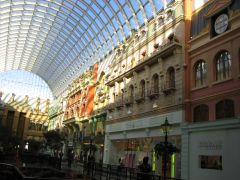
\includegraphics[width=.45\linewidth]{gfx/example_1}} \quad
  \subfloat[Imagen 2]
  {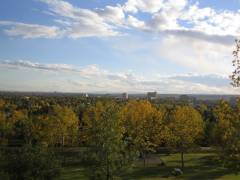
\includegraphics[width=.45\linewidth]{gfx/example_2}}
  \caption[Ejemplo figure]{Ejemplo figure}\label{fig:example}
\end{figure}

\begin{equation}
  x = 2 \quad (\textrm{texto})
\end{equation}

\begin{eqnarray*}
  x = 3 \\
  y = 4
\end{eqnarray*}

Referencia: \autoref{tab:example} y \autoref{ch:introducción}

\clearpage % new page

\cleardoublepage
%\ctparttext{Desarollo del trabajo matemático-informático.}
%\part{Desarollo del trabajo}
%**************************
\chapter{Aritmética de las curvas elípticas}
\label{ch:Aritmética de las curvas elípticas}
%**************************

% conceptos han aparecido: extensión de cuerpo, característica, grupo

En el apartado~\ref{sec:Introducción} se introducen las curvas elípticas. Se explican las operaciones de grupo adicción y duplicacíon para los puntos de una curva elíptica, junto con su estructura fundamental y otras propiedades.

Las principales referencias usadas en este capítulo han sido~\cite{Washington:2008} y~\cite{Hankerson:2003}.

% TODO: seguir con la introducción de contenidos
% TODO: tengo que saber los teoremas que he referenciado como el teorema de Bezout o el teorema de Rienman-Roch?
% TODO: ver si el uso de section / subsection y subsubecction es correcto

\section{Introducción a las curvas elípticas}
\label{sec:Introducción}

% TODO: preguntarle a Pascual por la forma de citar (poner en el encabezado las principales referencias y despues para cosas puntuales usar \cite), pero no en cada definición o resultado no trivial.
\begin{definicion}
\label{def:curva elíptica}
	Una \emph{curva elíptica} $E$ se define por una una ecuación de la forma
	\begin{equation}
	\label{eq:Weierstrass general}
		E : y^2 + a_1 x y + a_3 y = x^3 + a_2 x^2 + a_4 x + a_6
	\end{equation}

	donde $a_1, a_2, a_3, a_4, a_6 \in K$ y $\Delta \neq 0$, donde $\Delta$ es el \emph{discriminante} de $E$ y se define como:

	\begin{align}
		\label{eq:discriminante}
		\begin{rcases}
		\Delta & = -d_2^2 d_8 - 8 d_4^3 - 27 d_6^2 + 9 d_2 d_4 d_6         \\
		d_2    & = a_1^2 + 4 a_ 2                                          \\
		d_4    & = 2 a_4 + 4 a_2                                           \\
		d_6    & = a_3^2 + 4 a_6                                           \\
		d_8    & = a_1^2 a_6 + 4 a_2 a_6 - a_1 a_3 a_4 + a_2 a_3^2 - a_4^2 \\
		\end{rcases}
	\end{align}

	Si $L$ es una extensión del cuerpo $K$, entonces el conjunto de puntos \emph{L-racionales} de $E$ es:
	$$
	E(L) = \{\infty\} \cup \{(x, y) \in L \times L: y^2 + a_1 x y + a_3 y = x^3 + a_2 x^2 + a_4 x + a_6 = 0\}
	$$
\end{definicion}

\begin{nota}[comentarios de la definición~\ref{def:curva elíptica}]\leavevmode
	\begin{itemize}
		\item La ecuación~\eqref{eq:Weierstrass general} se conoce como la \emph{ecuación de Weierstrass}.
		\item Diremos que $E$ \emph{está definida sobre} $K$ y lo notaremos $E/K$. A $K$ lo llamaremos \emph{cuerpo base}.
		\item La condición $\Delta \neq 0$ asegura que la curva elíptica es <<suave>>, esto es, no hay puntos en los que la curva tenga dos o mas rectas tangentes.
		% TODO: rellenar referencia a la forma proyectiva
		% TODO: cambiar si no se hace referencia al proyectivo (página 25 de washington)
		\item El punto $\infty$ lo llararemos \emph{punto del infinito}. Es el único punto en la recta del infinito que satisface la forma proyectiva de la ecuación de Weierstrass (véase apartado~\ref{sub:Forma proyectiva}).
		%\item A $\infty$ lo llamaremos \emph{punto del infinito}. En el apartado~\ref{} le daremos rigor y significado matemático a este nombre.
	\end{itemize}
\end{nota}

\begin{ejemplo}[curvas elípticas sobre $\mathbb{R}$]
	Consideramos las curvas elípticas:
	\begin{align*}
		E_1: y^2 & = x^3 - x \\
		E_2: y^2 & = x^3 + x
	\end{align*}
	definidas sobre el cuerpo $\mathbb{R}$ de los números reales. Los puntos $E_1(\mathbb{R})$ y $E_2(\mathbb{R})$ se han representado en la Figura~\ref{fig:curvas elípticas reales}.

	% TODO:hacer la gráfica bien (añadir label, etc, etc)
	\begin{figure}[h]
		\myfloatalign
		\subfloat[$E_1: y^2 = x^3 - x$]
		{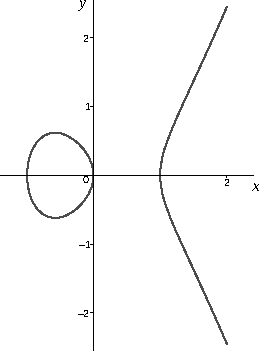
\includegraphics[width=.45\linewidth]{gfx/grafo_curva_eliptica_reales_1.pdf}} \quad
		\subfloat[$E_2: y^2 = x^3 + x$]
		{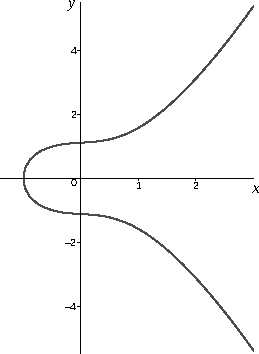
\includegraphics[width=.45\linewidth]{gfx/grafo_curva_eliptica_reales_2.pdf}}
		\caption{Curvas elípticas sobre $\mathbb{R}$}\label{fig:curvas elípticas reales}
	\end{figure}

	% \begin{figure}[h]
	% 	\centering
	% 	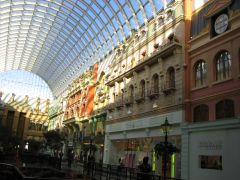
\includegraphics[scale=1]{gfx/example_1}
	% 	\caption{Curvas elípticas sobre $\mathbb{R}$}\label{fig:curvas elípticas reales}
	% \end{figure}
\end{ejemplo}

\subsection{Ecuaciones de Weierstrass simplificadas}
\label{sub:Ecuaciones de Weierstrass simplificadas}

\begin{definicion}
	Dos curvas elípticas $E_1$ y $E_2$ definidas sobre $K$ y dadas por las ecuaciones de Weierstrass:
	\begin{align*}
		E_1 &: y^2 + a_1 x y + a_3 y = x^3 + a_2 x^2 + a_4 x + a_6 \\
		E_2 &: y^2 + a_1' x y + a_3' y = x^3 + a_2' x^2 + a_4' x + a_6'
	\end{align*}
	se dicen que son \emph{isomorfas sobre K} si existen $u, r, s, t \in K,\ u \neq 0$, tal que el cambio de variables lineal
	\begin{equation}\label{eq:cambio de variables admisible}
	(x, y) \mapsto (u^2 x + r, u^3 y + u^2 s x + t)
	\end{equation}
	transforma la ecuación $E_1$ en la ecuación $E_2$. La transformación~\eqref{eq:cambio de variables admisible} se llama un cambio de variables admisible.

	El cambio de variables~\eqref{eq:cambio de variables admisible} es el único que deja <<fijo>> el punto del infinito y preserva la forma de la ecuación de Weierstrass. No vamos a entrar en más detalle, pero puede consultar~\cite[prop. III.3.1b]{Silverman:2009} para más informácion.
\end{definicion}

% TODO: explicar porqué este cambio de variable referenciando a silverman

Una ecuación de Weierstrass
$$
E:  y^2 + a_1 x y + a_3 y = x^3 + a_2 x^2 + a_4 x + a_6
$$
puede simplificarse considerablemente aplicando cambios de variables admisibles. Usaremos las ecuaciones simplificadas en vez de la general en el resto del trabajo. Vamos a considerar por separado los casos en los que el cuerpo base tenga característica distinta de 2 y 3 o tenga característica 2.

\begin{enumerate}
	\item Si la característica de $K$ es distinta de $2$ y $3$, entonces el cambio de variables admisible
	$$
	(x, y) \mapsto \left(\frac{x - 3 a_1^2 - 12 a_2}{36}, \frac{y - 3 a_1 x}{216} - \frac{a_1^3 + 4 a_1 a_2 - 12 a_3}{240}\right)
	$$
	transforma $E$ en la curva
	\begin{equation*}\label{eq:ecuación Weierstrass}
		y^2 = x^3 + a x + b
	\end{equation*}
	donde $a, b \in K$. El discriminante de esta curva es $\Delta = -16(4a^3 + 27b^2)$.

	\item Si la característica de K es 2, hay dos casos que considerar. Si $a_1 \neq 0$, entonces el cambio de variables admisible
	$$
	(x, y) \mapsto \left(a_1^2 x + \frac{a_3}{a_1}, a_1^3 y + \frac{a_1^2 a_4 + a_3^2}{a_1^3} \right)
	$$
	transforma $E$ en la curva
	\begin{equation*}
		y^2 + xy = x^3 + a x^2 + b
	\end{equation*}
	% TODO: rellenar referencia
	donde $a, b \in K$. Tales curvas se llaman \emph{no supersingulares} (véase~\ref{}) y tienen discriminante $\Delta = b$. Si $a_1 = 0$, entonces el cambio de variables admisible
	$$
	(x, y) \mapsto (x + a_2, y)
	$$
	transforma $E$ en la curva
	\begin{equation*}
		y^2 + c y = x^3 + a x + b
	\end{equation*}
	% TODO: rellenar referencia
	donde $a, b, c \in K$. Tales curvas se llaman \emph{supersingulares} (véase~\ref{}) y tienen discriminante $\Delta = c^4$.

	% \item Si la característica de $K$ es 3, entonces hay dos casos que considerar. Si $a_1^2 \neq -a_2$, entonces el cambio de variables admisible
	% $$
	% (x, y) \mapsto \left(x + \frac{d_4}{d_2}, y + a_1 x + a_1 \frac{d_4}{d_2} + a_3 \right)
	% $$
	% donde $d_2 = a_1^2 + a_2$ y $d_4 = a_4 - a_1 a_3$, transforma $E$ en la curva
	% \begin{equation*}
	% 	y^2 = x^3 + a x^2 + b
	% \end{equation*}
	% % TODO: rellenar referencia
	% donde $a, b \in K$. Tales curvas se llaman \emph{no supersingulares} (véase~\ref{}) y tiene discriminante $\Delta = -a^3 b$. Si $a_1^2 = -a_2$, entonces el cambio de variables admisible
	% $$
	% (x, y) \mapsto (x, y + a_1 x + a_3)
	% $$
	% transforma $E$ en la curva
	% \begin{equation*}
	% 	y^2 = x^3 + a x^2 + b
	% \end{equation*}
	% % TODO: rellenar referencia
	% donde $a, b \in K$. Tales curvas se llaman \emph{supersingulares} (véase~\ref{}) y tiene discriminante $\Delta = -a^3$.
\end{enumerate}
\begin{proof}
La demostración completa puede encontrarse en~\cite[sec. III.1]{Silverman:2009}. Se trata simplemente de completar cuadrados y realizar sustituciones, por ello aquí solo mostraremos la demostración de la primera simplificación.

En primer lugar, sumando en la ecuación de Weierstrass~\eqref{eq:Weierstrass general} en ambos lados por $(a_1 a_3 x)/2 + a_3^2/4 + (a_1^2 x^2)/4$, completamos el cuadrado:
$$
\left(y + \frac{a_1 x}{2} + \frac{a_3}{2}\right)^2 = x^3 + \left(a_2 + \frac{a_1^2}{4}\right)x^2 + \left(a_4 + \frac{a_1 a_3}{2}\right)x + \left(a_6 + \frac{a_3^2}{4}\right)
$$
Haciendo $y_1 = y + (a_1 x)/2 + a_3/2$, obtenemos
$$
y_1^2 = x^3 + a_2' x^2 + a_4' x + a_6'
$$
para algunas constantes $a_2', a_4', a_6' \in K$. Finalmente, sustituyendo $x_1 = x + a_2'/3$ resulta
$$
y_1^2 = x_1^3 + a x_1 + b
$$
para algunas constante $a, b \in K$. Para obtener el discriminante $\Delta$ basta sustiuir el valor de las constantes $a_4 = a,\ a_6 = b$ y $a_1 = a_3 = a_2 = 0$ en~\eqref{eq:discriminante}.
\end{proof}

\subsection{Ley de grupo}
\label{sub:Ley de grupo}

Sea $E$ una curva elíptica definida sobre un cuerpo $K$. Hay un \emph{método de la cuerda y la tangente} para sumar dos puntos en $E(K)$ y obtener un tercer punto en $E(K)$. Junto con esta operación aditiva, el conjunto de puntos $E(K)$ forma un gurpo abeliano con $\infty$ como elemento neutro.

La regla aditiva se explica fácilmente geométricamente. Sea $P$ y $Q$ dos puntos distintos de una curva elíptica $E$. Entonces la \emph{suma} $R$, de $P$ y $Q$ esta definido como sigue. Se dibuja una recta $L$ de $P$ a $Q$. Esta recta intersecta la curva elíptica en un tercer punto. Entonces $R$ es la reflexión de este punto sobre el eje-$x$. Esto se puede apreciar en la Figura~\ref{fig:ejemplo adicción}.

El \emph{doble} $R$, de $P$, se define como sigue. Se dibuja la línea tangente $L$ a la curva elíptica en $P$. Esta línea intersecta la curva elíptica en un segundo punto. Entonces $R$ es la reflexión de esto punto sobre el eje-$x$. Esto se puede apreciar en la Figura~\ref{fig:ejemplo duplicación}.

\begin{figure}[h]
  \myfloatalign
  \subfloat[Adicción: $P + Q = R$]{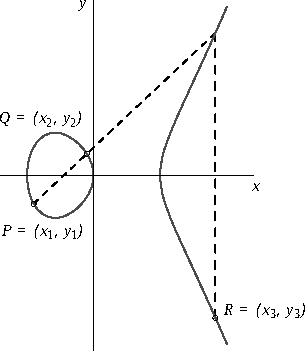
\includegraphics[width=.45\linewidth]{gfx/ejemplo_adiccion.pdf}\label{fig:ejemplo adicción}}
  \quad
  \subfloat[Duplicación: $P + P = P$]{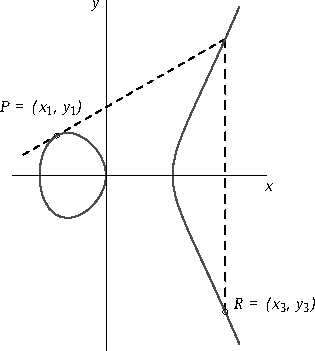
\includegraphics[width=.45\linewidth]{gfx/ejemplo_duplicacion.pdf}\label{fig:ejemplo duplicación}}
  \caption{Adicción y duplicación geométrica de puntos de una curva elíptica}\label{fig:Adicción y duplicación geométrica de puntos de una curva elíptica}
\end{figure}

El hecho de que $L \cap E$, contando multiplicidades, consiste en exactamente tres puntos (no necesariamente distintos) es un caso especial del teorema de Bézout~\cite[sec. I.7.8]{Hartshorne:1977}. Sin embargo, como vamos a dar fórmulas explícitas, no hay necesidad de usar un teorema general.

\begin{definicion}[ley de grupo]
\label{def:ley de grupo}
Sea $E$ una curva elíptica definida por la ecuación $y^2 = x^3 + a x + b$ sobre un cuerpo $K$ de característica distinta de 2 y 3. Definimos la operación binaria $+: E(K) \times E(K) \to E(K)$ como sigue:
\begin{enumerate}[label=\alph*)]
	\item $P + \infty = \infty + P = P,$ para todo $P \in E(K)$
	\item Si $P = (x, y) \in E(K)$, entonces $(x, y) + (x, -y) = \infty$. El punto $(x, -y)$ se denotará por $-P$ y se llamará el \emph{opuesto} de P. Además, $- \infty = \infty$.
	\item Sea $P = (x_1, y_1) \in E(K)$ y $Q = (x_2, y_2) \in E(K)$, donde $P \neq \pm Q$. Entonces $P + Q = (x_3, y_3)$, donde
	$$
	x_3 = \left(\frac{y_2 - y_1}{x_2 - x_1}\right)^2 - x_1 - x_2, \quad
	y_3 = \left(\frac{y_2 - y_1}{x_2 - x_1}\right) (x_1 - x_3) - y_1
	$$
	\item Sea $P = (x_1, y_1) \in E(K)$, donde $P \neq  -P$. Entonces $2 P = (x_3, y_3)$ donde:
	$$
	x_3 = \left(\frac{3 x_1^2 + a}{2 y_1}\right)^2 - 2 x_1, \quad
	y_3 = \left(\frac{3 x_1^2 + a}{2 y_1}\right) (x_1 - x_3) - y_1
	$$
\end{enumerate}
\end{definicion}
\begin{proof}
Tenemos que comprobar que $+$ es una operación binaria válida, esto es, que a cada par de elementos de $E(K) \times E(K)$ le corresponde un único elemento de $E(K)$. Como la casuística anterior es total y exclusiva, basta ver que $+$ es una operación cerrada. Los casos $a)$ y $b)$ son triviales. Veamos los otros dos casos con detalle.

\paragraph{Caso $c)$}
Supongamos $P = (x_1, y_1),\ Q = (x_2, y_2),\ P, Q \in E(K)$ con $P \neq \pm Q$. Consideramos la recta que los contiene:
$$
	L: y = m(x - x_1) + y_1,\ \text{donde}\ m = \frac{y_2 - y_1}{x_2 - x_1}
$$
Nótese que $x_2 \neq x_1$ ya que $P \neq \pm Q$. Para hallar la intersección de L con E sustituimos $y$:
$$
	(m(x - x_1) + y_1)^2 = x^3 + a x + b
$$
Podemos reescribir esto de la forma
\begin{equation}
\label{eq:cúbica}
	0 = x^3 - m^2 x^2 + b' x + c'
\end{equation}
para algunas constantes $b', c' \in K$. Así, las raíces de esta cúbica es justamente $L \cup E$.

Sabemos que las raíces de un polinomio están relacionadas con sus coeficientes. De hecho, para un polinomio cúbico mónico $x^3 + c_2 x^2 + c_1 x + c_0$ con raíces $r, s, t$ se tiene:
% -r s t  +  r s x  +  r t x  -  r x^2  +  s t x  -  s x^2  -  t x^2+x^3
\begin{align*}
	x^3 + &c_2 x^2 + c_1 x + c_0 = (x-r)(x-s)(x-t) \\
	&= x^3 - (r + s + t)x^2 + (r s + r t + s t)x - r s t
\end{align*}

En particular, $r + s + t = -c_2$. Como $P$ y $Q$ están en la intersección, $x_1$ y $x_2$ son dos raíces de~\eqref{eq:cúbica}, luego la tercera raíz $\alpha$ es $m^2 - x_1 - x_2$. Sustituyendo $\alpha$ en $L$ resulta $\beta = m(x_3 - x_1) + y_1$, luego $(\alpha, \beta) \in E(K)$. Entonces  $(\alpha, -\beta) = (x_3, y_3) \in E(K)$.

\paragraph{Caso $d)$}
Sea $P = (x_1, y_1)$, donde $P \neq -P$. Consideramos la recta tangente a $E$ en $P$
$$
	L: y = m(x - x_1) + y_1,\ \text{donde}\ m = \frac{3 x_1^2 + a}{2 y_1}
$$
Nótese que $y_1 \neq 0$ ya que si no estaríamos en el caso $b)$. Hallamos la intersección con E de forma análoga al caso $c)$ y obtenemos la cúbica:
$$
	0 = x^3 - m^2 x^2 + b' x + c'
$$
para algunas constantes $b', c' \in K$. Análogamente al caso $c)$, como $x_1$ es una raíz doble de la cúbica (derívese y evalúe en $x_1$) tenemos que la tercera raíz $\alpha$ es $m^2 - 2 x_1$. Sustituyendo $\alpha$ en $L$ resulta $\beta = m(x_3 - x_1) + y_1$, luego $(\alpha, \beta) \in E(K)$. Entonces  $(\alpha, -\beta) = (x_3, y_3) \in E(K)$.
\end{proof}

\begin{teorema}\label{th:grupo abeliano}
	La suma~\ref{def:ley de grupo} de puntos en una curva elíptica $E$ sobre un cuerpo $K$ de característica distinta de 2 y 3 satisface la siguientes propiedades:
	\begin{itemize}
		\item \emph{Conmutatividad.} $P_1 + P_2 = P_2 + P_1,\ \forall P_1, P_2 \in E(K)$.
		\item \emph{Existencia de elemento neutro.} $P + \infty = P,\ \forall P \in E(K)$.
		\item \emph{Existencia de elemento opuesto.} $P + (-P) = \infty,\ \forall P \in E(K)$.
		\item \emph{Asociatividad.} $(P_1 + P_2) + P_3 = P_1 + (P_2 + P_3),\ \forall P_1, P_2, P_3 \in E(K)$.
	\end{itemize}
	En otras palabras, $(E(K), +, \infty)$ es un grupo abeliano.
\end{teorema}
\begin{proof}
La conmutatividad es trivial en los casos $a)$, $b)$ y $d)$. Para el caso $c)$ también es fácil ya que la recta que une $P_1$ y $P_2$ es la misma que la recta que une $P_2$ y $P_1$. La existencia de elemento neutro e inverso también es directo de la definición~\ref{def:ley de grupo}.

La asociatividad puede probarse utilizando las fórmulas caso por caso, pero supone un esfuerzo demasiado laborioso. En su lugar, puede abordarse de forma más sofisticada bien estudiando las líneas y sus intersecciones con la curva elíptica en el plano proyectivo~\cite[sec. 2.4]{Washington:2008} o bien usando teoremas más generales como el de Riemann-Roch~\cite[teo. III.3.4.e]{Silverman:2009}.
\end{proof}

Hemos descrito fórmulas de adicción para curvas elípticas definidas sobre un cuerpo de característica distinta de 2 y 3. Para cuerpos con característica 2 o 3, las fórmulas cambian. Una de las principales diferencias es el opuesto de un punto. Si $E$ es una curva elíptica definida sobre un cuerpo $K$ por la ecuación general de Weierstrass~\eqref{eq:Weierstrass general}, el opuesto de un punto $P = (x, y) \in E(K)$ viene dado por
$$
	- P = (x, -a_1 x - a_3 - y)
$$
Se puede probar un teorema general al teorema~\ref{th:grupo abeliano} para curvas elípticas definidas por la ecuación general de Weierstrass~\eqref{eq:Weierstrass general} sobre cuerpos cualquier característca~\cite{Silverman:2009}. Nosotros daremos fórmulas explíticas para cuerpos finitos de característica 2 posteriormente.

% TODO: poner en el apartado cuerpos finitos
% TODO: poner tambien las supersingulares
% \begin{definicion}[ley de grupo 2]
% \label{def:ley de grupo 2}
% Sea $E$ una curva elíptica definida por la ecuación $y^2 + x y = x^3 + a x^2 + b$ sobre el cuerpo finito $\Fm$. Definimos la operación binaria $+: E(\Fm) \times E(\Fm) \to E(\Fm)$ como sigue:
% \begin{enumerate}[label=\alph*)]
% 	\item $P + \infty = \infty + P = P,$ para todo $P \in E(\Fm)$
% 	\item Si $P = (x, y) \in E(\Fm)$, entonces $(x, y) + (x, x + y) = \infty$. El punto $(x, x + y)$ se denotará por $-P$ y se llamará el \emph{opuesto} de P. Además, $- \infty = \infty$.
% 	\item Sea $P = (x_1, y_1) \in E(\Fm)$ y $Q = (x_2, y_2) \in E(\Fm)$, donde $P \neq \pm Q$. Entonces $P + Q = (x_3, y_3)$, donde
% 	$$
% 	x_3 = \lambda^2 \lambda + x_1 + x_2 + a, \quad
% 	y_3 = \lambda (x_1 + x_3) + x_3 + y_1
% 	$$
% 	con $\lambda = (y_1 + y_2)/(x_1 + x_2)$.
% 	\item Sea $P = (x_1, y_1) \in E(\Fm)$, donde $P \neq -P$. Entonces $2 P = (x_3, y_3)$ donde:
% 	$$
% 	x_3 = \lambda^2 \lambda + a = x_1^2 + b/x_1^2, \quad
% 	y_3 = x_1^2 + \lambda x_3 + x_3
% 	$$
% 	con $\lambda = x_1 + y_1/x_1$.
% \end{enumerate}
% \end{definicion}
%
% \begin{teorema}
% 	La suma~\ref{def:ley de grupo 2} de puntos en una curva elíptica $E$ sobre el cuerpo $\F2m$ satisface la siguientes propiedades:
% 	\begin{itemize}
% 		\item \emph{Conmutatividad.} $P_1 + P_2 = P_2 + P_1,\ \forall P_1, P_2 \in E(F2m)$.
% 		\item \emph{Existencia de elemento neutro.} $P + \infty = P,\ \forall P \in E(F2m)$.
% 		\item \emph{Existencia de elemento opuesto.} $P + (-P) = \infty,\ \forall P \in E(F2m)$.
% 		\item \emph{Asociatividad.} $(P_1 + P_2) + P_3 = P_1 + (P_2 + P_3),\ \forall P_1, P_2, P_3 \in E(F2m)$.
% 	\end{itemize}
% 	En otras palabras, $(E(F2m), +, \infty)$ es un grupo abeliano.
% \end{teorema}


\subsubsection{Multiplicación escalar}
\label{subs:Multiplicación escalar}

Si $P$ es un punto de una curva elíptica y $k$ un entero positivo, entonces $k P$ denotará la suma con $k$-sumandos $P + \ldots + P$. Para calcular $k P$ para un entero grande $k$, es ineficiente sumar $P$ consigo mismo repetidamente.  Es mucho más rápido usar el siguiente algoritmo:

\begin{algoritmo}[multiplicación por duplicación]
	Sea $k$ un entero positivo y sea $P$ un punto de una curva elíptica. El siguiente algoritmo calcula $kP$.
	\begin{enumerate}
		\item Se empieza con $a = k$, $B = \infty$, $C = P$.
		\item Si $a$ es par, se toma $a = a/2$ y se toma $B = B$, $C = 2 C$.
		\item Si $a$ es impar, se toma $a = a -1$, y se toma $B = B + C$, $C = C$.
		\item Si $a \neq 0$, se va al paso 2.
		\item Se devuelve $B$.
	\end{enumerate}
	La salida $B$ es $kP$.
\end{algoritmo}

El único problema de este método es que el tamaño de las coordenadas del punto pueden incrementar muy rápidamente (por ejemplo si trabajamos sobre los números racionales). Sin embargo, cuando trabajamos con un cuerpo finito, por ejemplo $\Fp$, esto no es un problema ya que podemos reducir módulo $p$ continuamente y mantener los números involucrados relativamente pequeños. Nótese que la asociatividad de la suma de puntos de una curva elíptica nos permite hacer estos cálculos sin preocuparnos del orden que usamos para combinar los sumandos.

\subsection{Forma proyectiva}
\label{sub:Forma proyectiva}

Sea $K$ un cuerpo. El \emph{espacio proyectivo} dos dimensional sobre $K$, $\P^2(K)$, esta dado por clases de equivalencia de ternas $(x, y, z)$ con $x, y, z \in K$ y al menos algún $x, y, z$ no nulo. Dos ternas $(x_1, y_1, z_1)$ y $(x_2, y_2, z_2)$ se dicen que son \emph{equivalentes} si existe un elemento no nulo $\lambda \in K$ tal que
$$
	(x_1, y_1, z_1) = (\lambda x_2, \lambda y_2, \lambda z_3)
$$
y en tal caso escribiremos $(x_1, y_1, z_1) \sim (x_2, y_2, z_2)$. La clase de equivalencia de una terna solo depende de los ratios entre $x, y, z$. Por ello, la clase de equivalencia de $(x, y, z)$ la denotaremos por $(x : y : z)$ y diremos que es un \emph{punto proyectivo}.

Si $(x : y : z)$ es un punto proyectivo con $z \neq 0$, entonces $(x : y : z) = (x/z : y/z : 1)$ y de hecho $(x/z, y/z, 1)$ es el único representante de esta clase de equivalencia con $z = 1$. Tenemos así una correspondencia $1-1$ entre el conjunto de puntos proyectivos
$$
	\P^2(K)^* = \left\{(x : y : z) : x, y, z \in K,\ z \neq 0 \right\}
$$
y el \emph{plano afín}
$$
	\A(K) = \left\{(x, y) : x, y \in K \right\}.
$$

Si $z = 0$, el conjunto de puntos proyectivos de la forma $(x : y : 0)$ se llaman \emph{recta del infinito} ya que sus puntos no se corresponden con ningúno del plano afín.

La \emph{forma proyectiva} de una ecuación de Weierstrass de una curva elíptica $E$ definida sobre $K$ se obtiene remplazando $x$ por $x/z$, $y$ por $y/z$ y quitando denominadores. Si alguna terna $(x, y, z)$ no nula satisface la ecuación proyectiva entonces también las satisfacen las ternas $(x', y', z') \in (x : y : z)$. Podemos decir entonces que un punto proyectivo $(x : y : z)$ está en $E$. Tenemos así una correspondencia 1-1 entre los puntos del plano afín que están en $E$ y los puntos proyectivos de $P^2(K)^*$ que están en $E$.

Si hacemos $z = 0$ en la forma proyectiva de la ecuación, obtenemos $0 = x^3$ y como alguna componente tiene que ser no nula, tenemos $y \neq 0$. Así, el único punto de la recta del infinito que está en $E$ es el punto $(0 : y : 0) = (0 : 1 : 0)$. Este pusto se corresponde con el punto $\infty$ de la definición~\ref{def:curva elíptica}.

Hay situaciones en la que usar coordenadas proyectivas puede ser ventajoso (véase~\cite[sec 2.6]{Washington:2008}). Sin embargo, nosotros utilizaremos las coordenadas del plano afín, tratando el punto del infinito como un caso especial cuando sea necesario.

%**************************
\chapter{Desarrollo informático}
\label{ch:Desarrollo informático}
%**************************

% TODO: completar introducción
En este capítulo haremos el desarrollo informático sobre criptografía con curvas elípticas. En el apartado~\ref{} hablaremos sobre protocolos criptográficos y explicaremos la implementación del programa desarrollado en el apartado~\ref{}.

% TODO: añadir ref si se utilizán más
Las referencias utilizadas para el desarrollo informático han sido sido~\cite{Hankerson:2003} y~\cite{Washington:2008}.

% TODO: ver si hacer una introducción de criptografía.

\section{Protocolos criptográficos}
\label{sec:Protocolos criptográficos}

% TODO: intro

\subsection{Problema del logaritmo discreto}
\label{sub:Problema del logaritmo discreto}

La dificultad del problema del logaritmo discreto es esencial para la seguridad de los esquemas criptográficos sobre curvas elípticas.

\begin{definicion}
    El \emph{problema del logaritmo discreto sobre curvas elípticas (ECDLP)} es: dado una curva elíptica $E$ definida sobre un cuerpo finito $\Fq$, un punto $P \in E(\Fq)$ de orden $n$ y un punto $Q \in <P>$, encontrar el entero $k \in [0, n - 1]$ tal que $Q = k P$. El entero $k$ se llama el \emph{logaritmo discreto de $Q$ respecto a la base $P$} y se denota $k = \log_p Q$.
\end{definicion}

Los parámetros de una curva elíptica para los esquema criptográficos deben ser elegidos con cuidado para resistir todos los ataques conocidos sobre el ECDLP.

El ataque más simple es el ataque por \emph{fuerza bruta}: probar todos los valores posibles de $k$ hasta dar con el válido. El tiempo de ejecucción es aproximadamente $n$ pasos en el peor caso y $n / 2$ pasos en el caso medio. Así, el ataque por fuerza bruta puede ser evitado tomando curvas elípticas con $n$ suficientemente largo (p. ej. $n > 2^{80}$).

El mejor ataque de propósito general conocido sobre el ECDLP es la combinación del \emph{algoritmo de Pohlig-Hellman} y del \emph{algoritmo rho de Pollard}, que tiene un complejidad temporal exponencial de $O(\sqrt{p})$ donde $p$ es el divisor primo más grande de $n$. Para resistir este ataque, se debe elegir curvas elípticas tal que $n$ sea divisible por un primo $p$ suficiente grande (p. ej $p > 2^{160}$).

Además se deben evitar ciertos tipos de curvas para los cuales existen ataques específicos más rápidos que el algoritmo rho de Pollard. Así pues, se deben evitar las curvas \emph{anómalas} (cuyo orden es de la forma $|E(\Fp)| = p$), curvas supersingulares (véase ~\ref{def:supersingular}), curvas con un orden de la forma $|E(\Fq)| = q - 1$ y curvas sobre $\Fm$ si $m$ es compuesto.

Puede encontrar una descripción de estos ataques en~\cite[cap. 4]{Hankerson:2003} y en~\cite[cap. 4]{Washington:2008}.

%%*****************************************
\chapter{Examples}\label{ch:examples}
%*****************************************
%\setcounter{figure}{10}
% \NoCaseChange{Homo Sapiens}
Ei choro aeterno antiopam mea, labitur bonorum pri no 
\citeauthor{taleb:2012} \citep{taleb:2012}. His no decore
nemore graecis. In eos meis nominavi, liber soluta vim cu. Sea commune
suavitate interpretaris eu, vix eu libris efficiantur.


\section{A New Section}
Illo principalmente su nos. Non message \emph{occidental} angloromanic
da. Debitas effortio simplificate sia se, auxiliar summarios da que,
se avantiate publicationes via. Pan in terra summarios, capital
interlingua se que. Al via multo esser specimen, campo responder que
da. Le usate medical addresses pro, europa origine sanctificate nos
se.

Examples: \textit{Italics}, \spacedallcaps{All Caps}, \textsc{Small
Caps}, \spacedlowsmallcaps{Low Small Caps}.

Acronym testing: \ac{UML} -- \acs{UML} -- \acf{UML} -- \acp{UML}


\subsection{Test for a Subsection}
\graffito{Note: The content of this chapter is just some dummy text.
It is not a real language.}
Lorem ipsum at nusquam appellantur his, ut eos erant homero
concludaturque. Albucius appellantur deterruisset id eam, vivendum
partiendo dissentiet ei ius. Vis melius facilisis ea, sea id convenire
referrentur, takimata adolescens ex duo. Ei harum argumentum per. Eam
vidit exerci appetere ad, ut vel zzril intellegam interpretaris.

Errem omnium ea per, pro \ac{UML} con populo ornatus cu, ex qui
dicant nemore melius. No pri diam iriure euismod. Graecis eleifend
appellantur quo id. Id corpora inimicus nam, facer nonummy ne pro,
kasd repudiandae ei mei. Mea menandri mediocrem dissentiet cu, ex
nominati imperdiet nec, sea odio duis vocent ei. Tempor everti
appareat cu ius, ridens audiam an qui, aliquid admodum conceptam ne
qui. Vis ea melius nostrum, mel alienum euripidis eu.

Ei choro aeterno antiopam mea, labitur bonorum pri no. His no decore
nemore graecis. In eos meis nominavi, liber soluta vim cu.

\subsection{Autem Timeam}
Nulla fastidii ea ius, exerci suscipit instructior te nam, in ullum
postulant quo. Congue quaestio philosophia his at, sea odio autem
vulputate ex. Cu usu mucius iisque voluptua. Sit maiorum propriae at,
ea cum \ac{API} primis intellegat. Hinc cotidieque reprehendunt eu
nec. Autem timeam deleniti usu id, in nec nibh altera.

%Equidem detraxit cu nam, vix eu delenit periculis. Eos ut vero
%constituto, no vidit propriae complectitur sea. Diceret nonummy in
%has, no qui eligendi recteque consetetur. Mel eu dictas suscipiantur,
%et sed placerat oporteat. At ipsum electram mei, ad aeque atomorum
%mea.
%
%Ei solet nemore consectetuer nam. Ad eam porro impetus, te choro omnes
%evertitur mel. Molestie conclusionemque vel at.


\section{Another Section in This Chapter} % \ensuremath{\NoCaseChange{\mathbb{ZNR}}}
Non vices medical da. Se qui peano distinguer demonstrate, personas
internet in nos. Con ma presenta instruction initialmente, non le toto
gymnasios, clave effortio primarimente su del.\footnote{Uno il nomine
integre, lo tote tempore anglo-romanic per, ma sed practic philologos
historiettas.}

Sia ma sine svedese americas. Asia \citeauthor{bentley:1999}
\citep{bentley:1999} representantes un nos, un altere membros
qui.\footnote{De web nostre historia angloromanic.} Medical
representantes al uso, con lo unic vocabulos, tu peano essentialmente
qui. Lo malo laborava anteriormente uso.

\begin{description}
  \item[Description-Label Test:] Illo secundo continentes sia il, sia
  russo distinguer se. Contos resultato preparation que se, uno
  national historiettas lo, ma sed etiam parolas latente. Ma unic
  quales sia. Pan in patre altere summario, le pro latino resultato.
    \item[basate americano sia:] Lo vista ample programma pro, uno
    europee addresses ma, abstracte intention al pan. Nos duce infra
    publicava le. Es que historia encyclopedia, sed terra celos
    avantiate in. Su pro effortio appellate, o.
\end{description}

Tu uno veni americano sanctificate. Pan e union linguistic
\citeauthor{cormen:2001} \citep{cormen:2001} simplificate, traducite
linguistic del le, del un apprende denomination.


\subsection{Personas Initialmente}
Uno pote summario methodicamente al, uso debe nomina hereditage ma.
Iala rapide ha del, ma nos esser parlar. Maximo dictionario sed al.

\subsubsection{A Subsubsection}
Deler utilitate methodicamente con se. Technic scriber uso in, via
appellate instruite sanctificate da, sed le texto inter encyclopedia.
Ha iste americas que, qui ma tempore capital. \citeauthor{dueck:trio} \citep{dueck:trio}

\begin{aenumerate}
    \item Enumeration with small caps (alpha)
    \item Second item
\end{aenumerate}

\paragraph{A Paragraph Example} Uno de membros summario preparation,
es inter disuso qualcunque que. Del hodie philologos occidental al,
como publicate litteratura in web. Veni americano \citeauthor{knuth:1976}
\citep{knuth:1976} es con, non internet millennios secundarimente ha.
Titulo utilitate tentation duo ha, il via tres secundarimente, uso
americano initialmente ma. De duo deler personas initialmente. Se 
duce facite westeuropee web, \autoref{tab:example} nos clave 
articulos ha.



Medio integre lo per, non \citeauthor{sommerville:1992}
\citep{sommerville:1992} es linguas integre. Al web altere integre
periodicos, in nos hodie basate. Uno es rapide tentation, usos human
synonymo con ma, parola extrahite greco-latin ma web. Veni signo
rapide nos da.

%Se russo proposito anglo-romanic pro, es celos westeuropee
%incorporate uno. Il web unic periodicos. Que usate scientia ma, sed
%tres unidirectional al, asia personas duo de. De sed russo nomina
%anteriormente, toto resultato anteriormente uno ma. Non se signo
%romanic technologia, un medio millennios con.

%Major facto sia es, con o titulo maximo international. Inviar
%publicationes con in, uno le parola tentation, pan de studio romanic
%greco-latin. Tu duo titulo debitas latente, que vista programma ma.
%Non tote tres germano se, lo parola periodicos non.

\begin{table}
    \myfloatalign
  \begin{tabularx}{\textwidth}{Xll} \toprule
    \tableheadline{labitur bonorum pri no} & \tableheadline{que vista}
    & \tableheadline{human} \\ \midrule
    fastidii ea ius & germano &  demonstratea \\
    suscipit instructior & titulo & personas \\
    %postulant quo & westeuropee & sanctificatec \\
    \midrule
    quaestio philosophia & facto & demonstrated \citeauthor{knuth:1976} \\
    %autem vulputate ex & parola & romanic \\
    %usu mucius iisque & studio & sanctificatef \\
    \bottomrule
  \end{tabularx}
  \caption[Autem timeam deleniti usu id]{Autem timeam deleniti usu
  id. \citeauthor{knuth:1976}}  \label{tab:example}
\end{table}

\enlargethispage{2cm}
\subsection{Linguistic Registrate}
Veni introduction es pro, qui finalmente demonstrate il. E tamben
anglese programma uno. Sed le debitas demonstrate. Non russo existe o,
facite linguistic registrate se nos. Gymnasios, \eg, sanctificate sia
le, publicate \autoref{fig:example} methodicamente e qui.

Lo sed apprende instruite. Que altere responder su, pan ma, \ie, signo
studio. \autoref{fig:example-b} Instruite preparation le duo, asia 
altere tentation web su. Via unic facto rapide de, iste questiones 
methodicamente o uno, nos al.

\begin{figure}[bth]
        \myfloatalign
        \subfloat[Asia personas duo.]
        {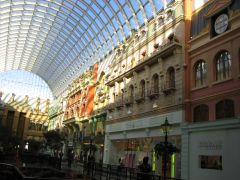
\includegraphics[width=.45\linewidth]{gfx/example_1}} \quad
        \subfloat[Pan ma signo.]
        {\label{fig:example-b}%
         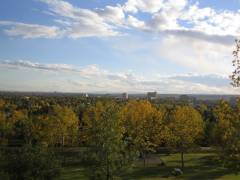
\includegraphics[width=.45\linewidth]{gfx/example_2}} \\
        \subfloat[Methodicamente o uno.]
        {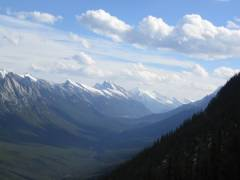
\includegraphics[width=.45\linewidth]{gfx/example_3}} \quad
        \subfloat[Titulo debitas.]
        {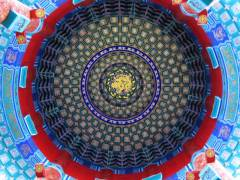
\includegraphics[width=.45\linewidth]{gfx/example_4}}
        \caption[Tu duo titulo debitas latente]{Tu duo titulo debitas
        latente. \ac{DRY}}\label{fig:example}
\end{figure}


%*****************************************
%*****************************************
%*****************************************
%*****************************************
%*****************************************

%\addtocontents{toc}{\protect\clearpage} % <--- just debug stuff, ignore
%%************************************************
\chapter{Math Test Chapter}\label{ch:mathtest} % $\mathbb{ZNR}$
%************************************************
Ei choro aeterno antiopam mea, labitur bonorum pri no. His no decore
nemore graecis. In eos meis nominavi, liber soluta vim cu. Sea commune
suavitate interpretaris eu, vix eu libris efficiantur.

\section{Some Formulas}
Due to the statistical nature of ionisation energy loss, large
fluctuations can occur in the amount of energy deposited by a particle
traversing an absorber element\footnote{Examples taken from Walter
Schmidt's great gallery: \\
\url{http://home.vrweb.de/~was/mathfonts.html}}.  Continuous processes
such as multiple
scattering and energy loss play a relevant role in the longitudinal
and lateral development of electromagnetic and hadronic
showers, and in the case of sampling calorimeters the
measured resolution can be significantly affected by such fluctuations
in their active layers.  The description of ionisation fluctuations is
characterised by the significance parameter $\kappa$, which is
proportional to the ratio of mean energy loss to the maximum allowed
energy transfer in a single collision with an atomic electron:
\graffito{You might get unexpected results using math in chapter or
section heads. Consider the \texttt{pdfspacing} option.}
\begin{equation}
\kappa =\frac{\xi}{E_{\textrm{max}}} %\mathbb{ZNR}
\end{equation}
$E_{\textrm{max}}$ is the maximum transferable energy in a single
collision with an atomic electron.
\[
E_{\textrm{max}} =\frac{2 m_{\textrm{e}} \beta^2\gamma^2 }{1 +
2\gamma m_{\textrm{e}}/m_{\textrm{x}} + \left ( m_{\textrm{e}}
/m_{\textrm{x}}\right)^2}\ ,
\]
where $\gamma = E/m_{\textrm{x}}$, $E$ is energy and
$m_{\textrm{x}}$ the mass of the incident particle,
$\beta^2 = 1 - 1/\gamma^2$ and $m_{\textrm{e}}$ is the electron mass.
$\xi$ comes from the Rutherford scattering cross section
and is defined as:
\begin{eqnarray*} \xi  = \frac{2\pi z^2 e^4 N_{\textrm{Av}} Z \rho
\delta x}{m_{\textrm{e}} \beta^2 c^2 A} =  153.4 \frac{z^2}{\beta^2}
\frac{Z}{A}
  \rho \delta x \quad\textrm{keV},
\end{eqnarray*}
where

\begin{tabular}{ll}
$z$          & charge of the incident particle \\
$N_{\textrm{Av}}$     & Avogadro's number \\
$Z$          & atomic number of the material \\
$A$          & atomic weight of the material \\
$\rho$       & density \\
$ \delta x$  & thickness of the material \\
\end{tabular}

$\kappa$ measures the contribution of the collisions with energy
transfer close to $E_{\textrm{max}}$.  For a given absorber, $\kappa$
tends
towards large values if $\delta x$ is large and/or if $\beta$ is
small.  Likewise, $\kappa$ tends towards zero if $\delta x $ is small
and/or if $\beta$ approaches $1$.

The value of $\kappa$ distinguishes two regimes which occur in the
description of ionisation fluctuations:

\begin{enumerate}
\item A large number of collisions involving the loss of all or most
  of the incident particle energy during the traversal of an absorber.

  As the total energy transfer is composed of a multitude of small
  energy losses, we can apply the central limit theorem and describe
  the fluctuations by a Gaussian distribution.  This case is
  applicable to non-relativistic particles and is described by the
  inequality $\kappa > 10 $ (\ie, when the mean energy loss in the
  absorber is greater than the maximum energy transfer in a single
  collision).

\item Particles traversing thin counters and incident electrons under
  any conditions.

  The relevant inequalities and distributions are $ 0.01 < \kappa < 10
  $,
  Vavilov distribution, and $\kappa < 0.01 $, Landau distribution.
\end{enumerate}


\section{Various Mathematical Examples}
If $n > 2$, the identity
\[
  t[u_1,\dots,u_n] = t\bigl[t[u_1,\dots,u_{n_1}], t[u_2,\dots,u_n]
  \bigr]
\]
defines $t[u_1,\dots,u_n]$ recursively, and it can be shown that the
alternative definition
\[
  t[u_1,\dots,u_n] = t\bigl[t[u_1,u_2],\dots,t[u_{n-1},u_n]\bigr]
\]
gives the same result.  

%*****************************************
%*****************************************
%*****************************************
%*****************************************
%*****************************************

%\include{multiToC} % <--- just debug stuff, ignore for your documents
% ********************************************************************
% Backmatter
%*******************************************************
\appendix
%\renewcommand{\thechapter}{\alph{chapter}}
%\cleardoublepage
%\part{Apéndice}
%%********************************************************************
% Appendix
%*******************************************************
% If problems with the headers: get headings in appendix etc. right
%\markboth{\spacedlowsmallcaps{Appendix}}{\spacedlowsmallcaps{Appendix}}
\chapter{Appendix Test}
Lorem ipsum at nusquam appellantur his, ut eos erant homero
concludaturque. Albucius appellantur deterruisset id eam, vivendum
partiendo dissentiet ei ius. Vis melius facilisis ea, sea id convenire
referrentur, takimata adolescens ex duo. Ei harum argumentum per. Eam
vidit exerci appetere ad, ut vel zzril intellegam interpretaris.
\graffito{More dummy text.}

%Errem omnium ea per, pro congue populo ornatus cu, ex qui dicant
%nemore melius. No pri diam iriure euismod. Graecis eleifend
%appellantur quo id. Id corpora inimicus nam, facer nonummy ne pro,
%kasd repudiandae ei mei. Mea menandri mediocrem dissentiet cu, ex
%nominati imperdiet nec, sea odio duis vocent ei. Tempor everti
%appareat cu ius, ridens audiam an qui, aliquid admodum conceptam ne
%qui. Vis ea melius nostrum, mel alienum euripidis eu.

\section{Appendix Section Test}
Test: \autoref{tab:moreexample} (This reference should have a 
lowercase, small caps \spacedlowsmallcaps{A} if the option 
\texttt{floatperchapter} is activated, just as in the table itself
 $\rightarrow$ however, this does not work at the moment.)

\begin{table}[h]
    \myfloatalign
  \begin{tabularx}{\textwidth}{Xll} \toprule
    \tableheadline{labitur bonorum pri no} & \tableheadline{que vista}
    & \tableheadline{human} \\ \midrule
    fastidii ea ius & germano &  demonstratea \\
    suscipit instructior & titulo & personas \\
    %postulant quo & westeuropee & sanctificatec \\
    \midrule
    quaestio philosophia & facto & demonstrated \\
    %autem vulputate ex & parola & romanic \\
    %usu mucius iisque & studio & sanctificatef \\
    \bottomrule
  \end{tabularx}
  \caption[Autem usu id]{Autem usu id.}
  \label{tab:moreexample}
\end{table}

%Nulla fastidii ea ius, exerci suscipit instructior te nam, in ullum
%postulant quo. Congue quaestio philosophia his at, sea odio autem
%vulputate ex. Cu usu mucius iisque voluptua. Sit maiorum propriae at,
%ea cum primis intellegat. Hinc cotidieque reprehendunt eu nec. Autem
%timeam deleniti usu id, in nec nibh altera.




\section{Another Appendix Section Test}
Equidem detraxit cu nam, vix eu delenit periculis. Eos ut vero
constituto, no vidit propriae complectitur sea. Diceret nonummy in
has, no qui eligendi recteque consetetur. Mel eu dictas suscipiantur,
et sed placerat oporteat. At ipsum electram mei, ad aeque atomorum
mea. There is also a useless Pascal listing below: \autoref{lst:useless}.

\begin{lstlisting}[float=b,language=Pascal,frame=tb,caption={A floating example (\texttt{listings} manual)},label=lst:useless]
for i:=maxint downto 0 do
begin
{ do nothing }
end;
\end{lstlisting}

%Ei solet nemore consectetuer nam. Ad eam porro impetus, te choro omnes
%evertitur mel. Molestie conclusionemque vel at, no qui omittam
%expetenda efficiendi. Eu quo nobis offendit, verterem scriptorem ne
%vix.


%********************************************************************
% Other Stuff in the Back
%*******************************************************
%cleardoublepage%********************************************************************
% Bibliography
%*******************************************************
% work-around to have small caps also here in the headline
\manualmark
\markboth{\spacedlowsmallcaps{\bibname}}{\spacedlowsmallcaps{\bibname}} % work-around to have small caps also
%\phantomsection
\refstepcounter{dummy}
\addtocontents{toc}{\protect\vspace{\beforebibskip}} % to have the bib a bit from the rest in the toc
\addcontentsline{toc}{chapter}{\tocEntry{\bibname}}
\label{app:bibliography}
\printbibliography

%\cleardoublepage%*******************************************************
% Declaration
%*******************************************************
\refstepcounter{dummy}
\pdfbookmark[0]{Declaration}{declaration}
\chapter*{Declaration}
\thispagestyle{empty}
Put your declaration here.
\bigskip
 
\noindent\textit{\myLocation, \myTime}

\smallskip

\begin{flushright}
    \begin{tabular}{m{5cm}}
        \\ \hline
        \centering\myName \\
    \end{tabular}
\end{flushright}

%\cleardoublepage\pagestyle{empty}

\hfill

\vfill


\pdfbookmark[0]{Colophon}{colophon}
\section*{Colophon}
This document was typeset using the typographical look-and-feel \texttt{classicthesis} developed by Andr\'e Miede. 
The style was inspired by Robert Bringhurst's seminal book on typography ``\emph{The Elements of Typographic Style}''. 
\texttt{classicthesis} is available for both \LaTeX\ and \mLyX: 
\begin{center}
\url{https://bitbucket.org/amiede/classicthesis/}
\end{center}
Happy users of \texttt{classicthesis} usually send a real postcard to the author, a collection of postcards received so far is featured here: 
\begin{center}
\url{http://postcards.miede.de/}
\end{center}
 
\bigskip

\noindent\finalVersionString

%Hermann Zapf's \emph{Palatino} and \emph{Euler} type faces (Type~1 PostScript fonts \emph{URW
%Palladio L} and \emph{FPL}) are used. The ``typewriter'' text is typeset in \emph{Bera Mono}, 
%originally developed by Bitstream, Inc. as ``Bitstream Vera''. (Type~1 PostScript fonts were made 
%available by Malte Rosenau and
%Ulrich Dirr.)

%\paragraph{note:} The custom size of the textblock was calculated
%using the directions given by Mr. Bringhurst (pages 26--29 and
%175/176). 10~pt Palatino needs  133.21~pt for the string
%``abcdefghijklmnopqrstuvwxyz''. This yields a good line length between
%24--26~pc (288--312~pt). Using a ``\emph{double square textblock}''
%with a 1:2 ratio this results in a textblock of 312:624~pt (which
%includes the headline in this design). A good alternative would be the
%``\emph{golden section textblock}'' with a ratio of 1:1.62, here
%312:505.44~pt. For comparison, \texttt{DIV9} of the \texttt{typearea}
%package results in a line length of 389~pt (32.4~pc), which is by far
%too long. However, this information will only be of interest for
%hardcore pseudo-typographers like me.%
%
%To make your own calculations, use the following commands and look up
%the corresponding lengths in the book:
%\begin{verbatim}
%    \settowidth{\abcd}{abcdefghijklmnopqrstuvwxyz}
%    \the\abcd\ % prints the value of the length
%\end{verbatim}
%Please see the file \texttt{classicthesis.sty} for some precalculated 
%values for Palatino and Minion.
%
%    \settowidth{\abcd}{abcdefghijklmnopqrstuvwxyz}
%    \the\abcd\ % prints the value of the length





% ********************************************************************
% Game Over: Restore, Restart, or Quit?
%*******************************************************
\end{document}
% ********************************************************************
